%-------------------------------------------------------------------------------
\section{Event Selection}
\label{sec:eventPreselection}
%-------------------------------------------------------------------------------
This analysis is based on data collected by the ATLAS experiment in
$pp$ collisions at $\sqrt{s}=8\tev$
between April and October 2012. The corresponding integrated
luminosity is $20.2~\ifb$.
Only events collected using
a single electron or single muon trigger under stable beam conditions and for which
all detector subsystems were fully operational were considered.
%The exact details of the trigger used varied with the data taking period under consideration.
%For the dataset at  $\sqrt{s}=7\tev$, the $\pt$ thresholds are 18~\gev\ for
%muons and 20 or 22~\gev\ for electrons.  In later stages, the 22~\gev\
%electron trigger was supplemented with a higher-$\pt$ trigger with a
%threshold of 45~\gev\  to improve the efficiency at high instantaneous
%luminosity.

The $\pt$ thresholds are 24 or 60~\gev\ for
electrons (logical OR of EF\_e24vhi\_medium1 and EF\_e60\_medium1 trigger chains) and 24 or 36~\gev\ 
for muons (logical OR of EF\_mu24i\_tight and EF\_mu36\_tight trigger chains).  
The triggers with the lower $\pt$ threshold include isolation requirements on the candidate lepton, 
resulting in inefficiencies at high $\pt$
that are recovered by the triggers with higher $\pt$ threshold.
The triggers use similar but looser selection criteria than the final reconstruction
requirements.
% and reach a plateau at 25~\gev\ (electrons) and 20~\gev\ (muons).

Events passing the trigger are required to have at least one reconstructed vertex with at least five associated tracks, consistent with the beam collision region in the $x-y$ plane. If more than one vertex is found, the primary vertex is taken to be the vertex with the largest scalar sum of transverse momenta from its associated tracks. Events are discarded if any jet with $\pt > 20\gev$ is independently identified as out-of-time activity from a previous $pp$ collision or as calorimeter noise~\cite{ref:ATLAS-CONF-2012-020}.

In order to pick up semileptonic \ttbar decays, events are required to have exactly one
reconstructed electron or muon with \pt$>25$ \gev\ and at least four jets satisfying the
quality and kinematic criteria discussed in Section~\ref{sec:jetObjectDef8TeV}. The remaining events are separated into two independent \bt tag regions: one with exactly one \bt tag and one with two or more \bt tags. For both electron and muon channels, the selected lepton is required to match ($\Delta R < 0.15$) the lepton reconstructed by the high-level trigger.
%Events are vetoed if they contain a selected electron which shares an
%inner detector track with a reconstructed muon passing all constraints
%except the muon-jet separation requirement.  The event must contain
%exactly one selected charged lepton and at least 4 jets.

Since the background from multi-jet production is very small in the high
jet and \bt tag multiplicity regions which are the focus of this analysis, no requirements on the $\met$
or transverse mass of the \w boson are applied for the inclusive region with 2 or more \bt tags. In the 1 exclusive \bt tag region, the \met is required to be greater than 20 GeV and the sum of \met and transverse mass of the leptonic \w boson is required to be greater than 60 GeV in order to suppress multi-jet (QCD) backgrounds coming from the presence of misidentified leptons.

% modified by Gvantsa
%In the di-lepton channel, events are required to have exactly two
%leptons of opposite charge and at least two jets, at least one of which
%is \bt tagged. The leading and sub-leading leptons should have \pt$>25$ \gev . In this channel, events can be further categorized according to the lepton flavour into $ee$,
%$\mu\mu$ and $e\mu$ samples. The scalar sum of the transverse energy
%of leptons and jets, $H_T$ , is calculated in the $e\mu$ category and
%required to be above 130~\gev. This cut is not applied in the $ee$ and
%$\mu\mu$ event categories, but in this case to suppress backgrounds  from
%Z+jets events in the missing transverse energy must satisfy $\ET_{miss} >$30 GeV, and the invariant mass of the two leptons must differ by at least 10 \gev from the Z boson mass, i.e.
% $| \ m_{ll} - m_Z| > 10$~\gev.
% modified by Gvantsa

Selected events are categorized into 1 exclusive and 2 \bt tag inclusive regions. Event yields for both lepton channels and \bt tag regions are shown in Table \ref{tab:event_yield}. Cutting on the log likelihood (discussed in Sec. \ref{sec:hadronicOptimization}) significantly reduces background contributions and improves the data/prediction agreement. Studies on optimizing the sensitivity of the \w helicity measurement using a cut on the likelihood are presented in Sec. \ref{sec:hadronicOptimization}. %Plots showing data/prediction comparisons after event selection for both lepton channels and \bt tag regions are shown in Figures \ref{fig:control_plots_el_1excl}-\ref{fig:control_plots_mu_2incl}. All control plots except for log likelihood and event probability are shown after the log likelihood cut.
Plots showing data/prediction comparisons after event selection and log likelihood cut for both lepton channels and \bt tag regions are shown in Figures \ref{fig:control_plots_el_1excl}-\ref{fig:control_plots_mu_2incl}. Control plots for the pre-fit $cos\theta^*$ distributions are shown in Figure \ref{fig:control_plots_costheta} for both the 2 inclusive and 1 exclusive \bt tag regions.

The largest shape difference between the leptonic and hadronic angles in Figure~\ref{fig:control_plots_costheta} is due to the fact that for events with $\cos \theta^{*} \sim -1$, the charged lepton (down-type quark) is emitted parallel to the \bt-jet, and more leptonic events fail the lepton \pt and lepton-\bt-jet isolation requirements imposed by the event selection. This affects the leptonic side more than the hadronic side since there is no corresponding jet-\bt-jet isolation requirement. Another noticeable difference between the 1 exclusive and 2 inclusive shapes around $\cos \theta^{*} \sim +1$ is where the neutrino (up-type quark) and \bt-jet are parallel in the mother \w boson rest frame, so the MET cut in the 1 exclusive region causes some events to fail the selection criteria. Lastly, the hadronic $\cos \theta^{*}$ distribution in the 1 exclusive region suffers from an additional light jet/\bt-jet quark mismatch which results in the double peak structure.

\begin{table}
\centering 
\begin{tabular}{c|c|c|c|c}
\hline
e+jets & \multicolumn{2}{c|}{No Likelihood Cut} & \multicolumn{2}{c}{Log(Likelihood) $>$ -48} \\\hline
Sample & 1 \bt tag & $\geq2$ \bt tags & 1 \bt tag & $\geq2$ \bt tags \\
\hline
%\ttbar     &  71711.4$\pm$ XXX  &  75853.6$\pm$ XXX  & 36494 $\pm$ xxx & 36028 $\pm$ xxx \\
%QCD        &  11830.8$\pm$ XXX  &  6236.09$\pm$ XXX  & 1996 $\pm$ xxx & 974 $\pm$ xxx \\
%\w + jets &  xxx$\pm$ xxx  &  xxx$\pm$ xxx  & 4540 $\pm$ xxx & 615 $\pm$ xxx \\
%$Z$ + jets &  3846.93$\pm$ XXX  &  1280.75$\pm$ XXX  &  1200  $\pm$ xxx & 329 $\pm$ xxx \\
%Single top &  5552.51$\pm$ XXX  &  3682.33$\pm$ XXX  & 215 $\pm$ xxx & 33 $\pm$ xxx \\
%Diboson    &  808.452$\pm$ XXX  &  175.565$\pm$ XXX  & 4684 $\pm$ xxx &  2449  $\pm$ xxx \\
%\hline
%Total expected    &  109093$\pm$ XXX  &  89526$\pm$ XXX  & 49128 $\pm$ xxx & 40428 $\pm$ xxx \\
%\hline
%Data       &   102591        &     89414   &  45246  & 40045\\
\ttbar     		&  69822 	$\pm$ 4490  &  74467 	$\pm$ 4788  & 36495 	$\pm$ 2347 	& 36028 $\pm$ 2317 \\
Single top 		&  5553 	$\pm$ 944  	&  3682 	$\pm$ 626  	& 1996 	$\pm$ 339 	& 974 	$\pm$ 166 \\
$W$ + light 	&  2498 	$\pm$ 125  	&  104 		$\pm$ 7  	& 600 	$\pm$ 30 	& 24 	$\pm$ 1 \\
$W$ + c 		&  4490 	$\pm$ 1123  &  274 		$\pm$ 64  	& 1212 	$\pm$ 303 	& 54 	$\pm$ 13 \\
$W$ + bb/cc 	&  12040 	$\pm$ 843  	&  2866 	$\pm$ 134  	& 2726 	$\pm$ 191 	& 538 	$\pm$ 38 \\
$Z$ + jets 		&  3847 	$\pm$ 1847  &  1281 	$\pm$ 615  	& 1200  	$\pm$ 576 	& 329 	$\pm$ 158 \\
Diboson    		&  808 		$\pm$ 388  	&  176 		$\pm$ 84  	& 215 	$\pm$ 103 	& 33  	$\pm$ 16 \\
QCD        		&  6862 	$\pm$ 2059  &  2054 	$\pm$ 616  & 2272 	$\pm$ 682 	& 447 	$\pm$ 134 \\
\hline
Total expected  &  105920 	$\pm$ 5553  &  84904 	$\pm$ 4871  & 46716 $\pm$ 2561	& 38426 $\pm$ 2332 \\
\hline
Data       	&   102591	            &  89414 	            & 45246       	& 40045            \\
\hline
Dev. \% 	&	3.2 				& -5.0 					& 3.2 			& -4.0 \\
\hline\hline
\end{tabular}
%\end{table}

\vspace{7.5mm}
%\begin{table}
%\centering
\begin{tabular}{c|c|c|c|c}
\hline
$\mu$+jets & \multicolumn{2}{c|}{No Likelihood Cut} & \multicolumn{2}{c}{Log(Likelihood) $>$ -48} \\\hline
Sample & 1 \bt tag & $\geq2$ \bt tags & 1 \bt tag & $\geq2$ \bt tags \\
\hline
%\ttbar     &  87695.6$\pm$ XXX  &  91879.4$\pm$ XXX  &  43597  $\pm$ xxx &  42634 $\pm$ xxx \\
%QCD        &  7447.08$\pm$ XXX  &  3341.7$\pm$ XXX &  2328  $\pm$ xxx &  1102  $\pm$ xxx \\
%\w + jets &  xxx$\pm$ XXX  &  xxx$\pm$ XXX &  5720  $\pm$ xxx &  876  $\pm$ xxx \\
%$Z$ + jets &  2224.07$\pm$ XXX  &  695.335$\pm$ XXX & 606 $\pm$ xxx &   158  $\pm$ xxx \\
%Single top &  6717.23$\pm$ XXX  &  4463.87$\pm$ XXX & 214 $\pm$ xxx & 37 $\pm$ xxx \\
%Diboson    &  924.06$\pm$ XXX  &  185.292$\pm$ XXX & 2796 $\pm$ xxx &  1159  $\pm$ xxx \\
%\hline
%Total expected    &  125243$\pm$ XXX  &  103827$\pm$ XXX & 55261 $\pm$ xxx & 45965 $\pm$ xxx \\
%\hline
%Data       &   126333        &     108131   & 53747 & 46048 \\
\ttbar     		&  87405 	$\pm$ 5620  &  92321 	$\pm$ 5936  & 43597 $\pm$ 2803 	& 42634 $\pm$ 2741 \\
Single top 		&  6717 	$\pm$ 1142  &  4464 	$\pm$ 759  & 2328 	$\pm$ 396 	& 1102 	$\pm$ 187 \\
$W$ + light 	&  3296 	$\pm$ 165  &  177 		$\pm$ 11  & 761 	$\pm$ 38 	& 45 	$\pm$ 2 \\
$W$ + c 		&  5556 	$\pm$ 1389  &  329 		$\pm$ 77  & 1439 	$\pm$ 360 	& 51 	$\pm$ 13 \\
$W$ + bb/cc 	&  16386 	$\pm$ 1147  &  4098 		$\pm$ 191  & 3520 	$\pm$ 246 	& 780 	$\pm$ 55 \\
$Z$ + jets 		&  2445 	$\pm$ 1174  &  744 		$\pm$ 357  & 606  	$\pm$ 291 	& 158 	$\pm$ 76 \\
Diboson    		&  924 		$\pm$ 444  &  185 		$\pm$ 89  & 214 	$\pm$ 103 	& 37  	$\pm$ 18 \\
QCD        		&  5280 	$\pm$ 1584  &  1457 	$\pm$ 437  & 1746 	$\pm$ 524 	& 323 	$\pm$ 97 \\
\hline
Total expected  &  128009 	$\pm$ 6344  &  103775 	$\pm$ 6019  & 54211 	$\pm$ 2928	& 45130 $\pm$ 2751 \\			
\hline
Data       	&   126333	            &  108131 	            & 53747      	        &  46048         \\
\hline
Dev. \% 	&	1.3 				& -4.0 					& 0.9 			& -2.0 \\
\hline\hline
\end{tabular}
\caption{Event yields in the electron (top) and muon channel (bottom) for 1 exclusive and 2 inclusive \bt tag regions after event selection. Errors on the Monte Carlo yields come from the uncertainties in the normalization of each sample. The last two columns refers to the yields after applying the likelihood cut. Details are given in \ref{sec:hadronicOptimization}}% combined in quadrature with the statistical uncertainty on the Monte Carlo yield.}
\label{tab:event_yield}
\end{table}


\begin{figure}[!hb]
\begin{center}

		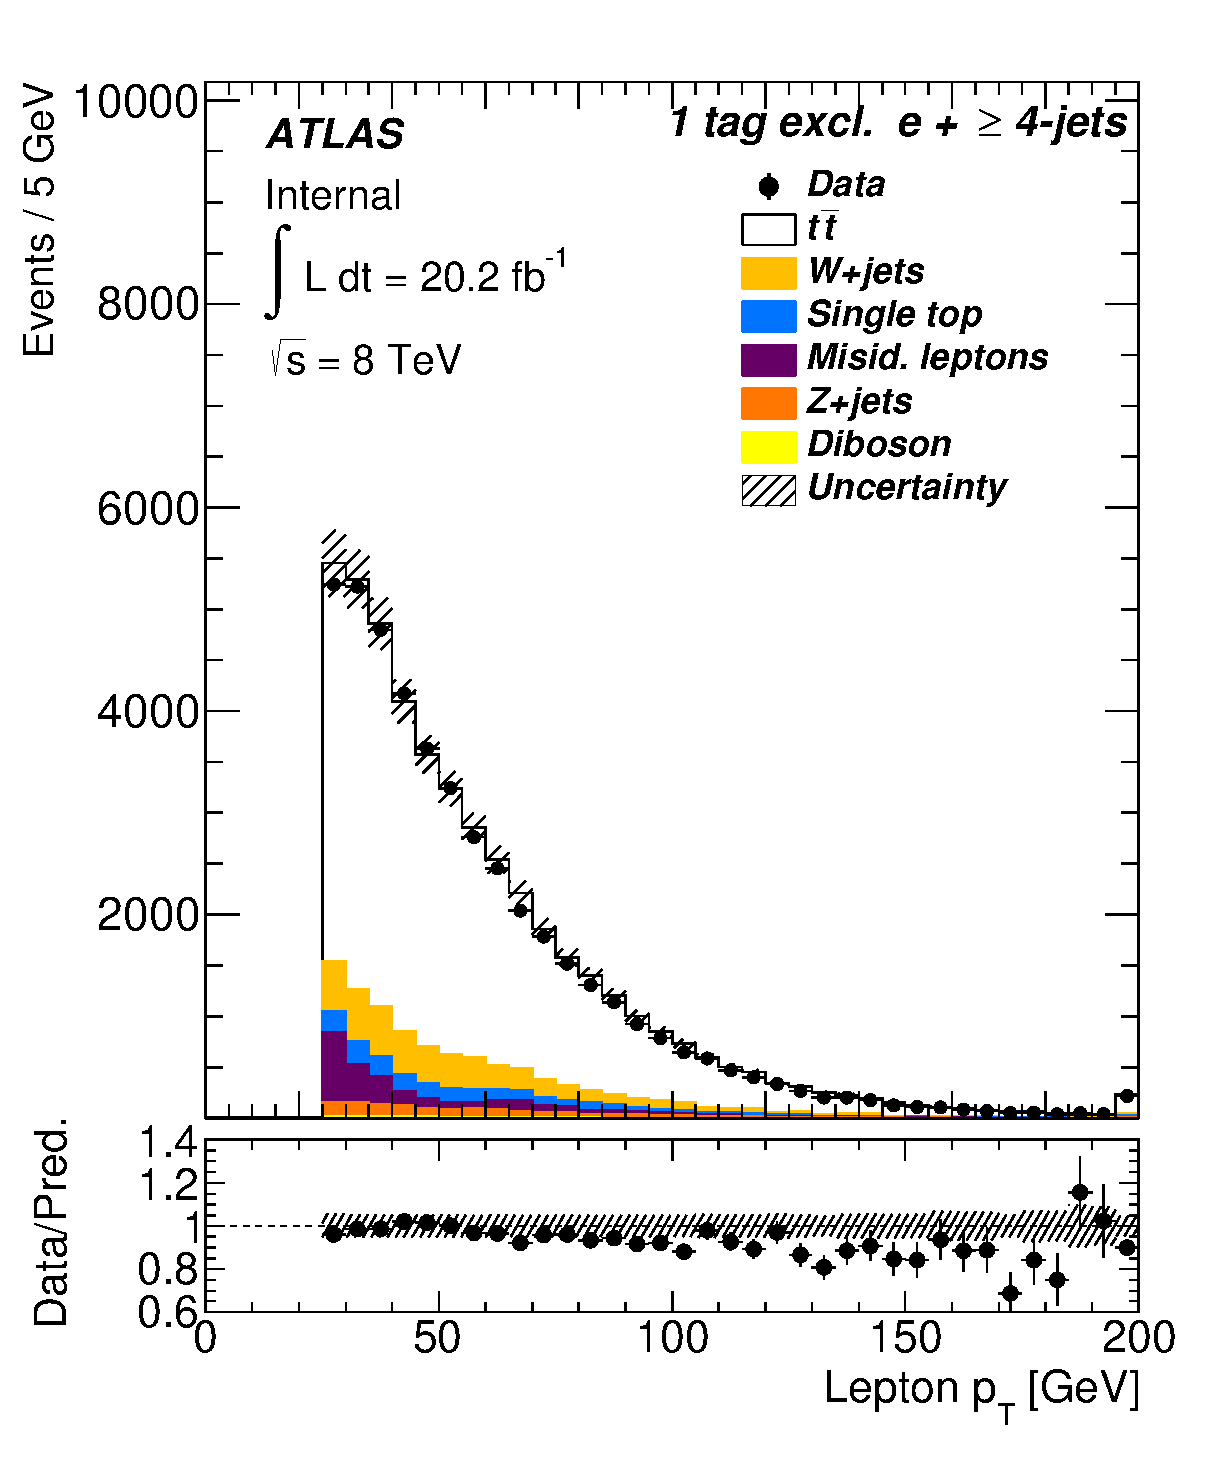
\includegraphics[height=65mm]{chapters/whel/figures/control_Plots2/bTag_1excl/LeptonPt_el}
		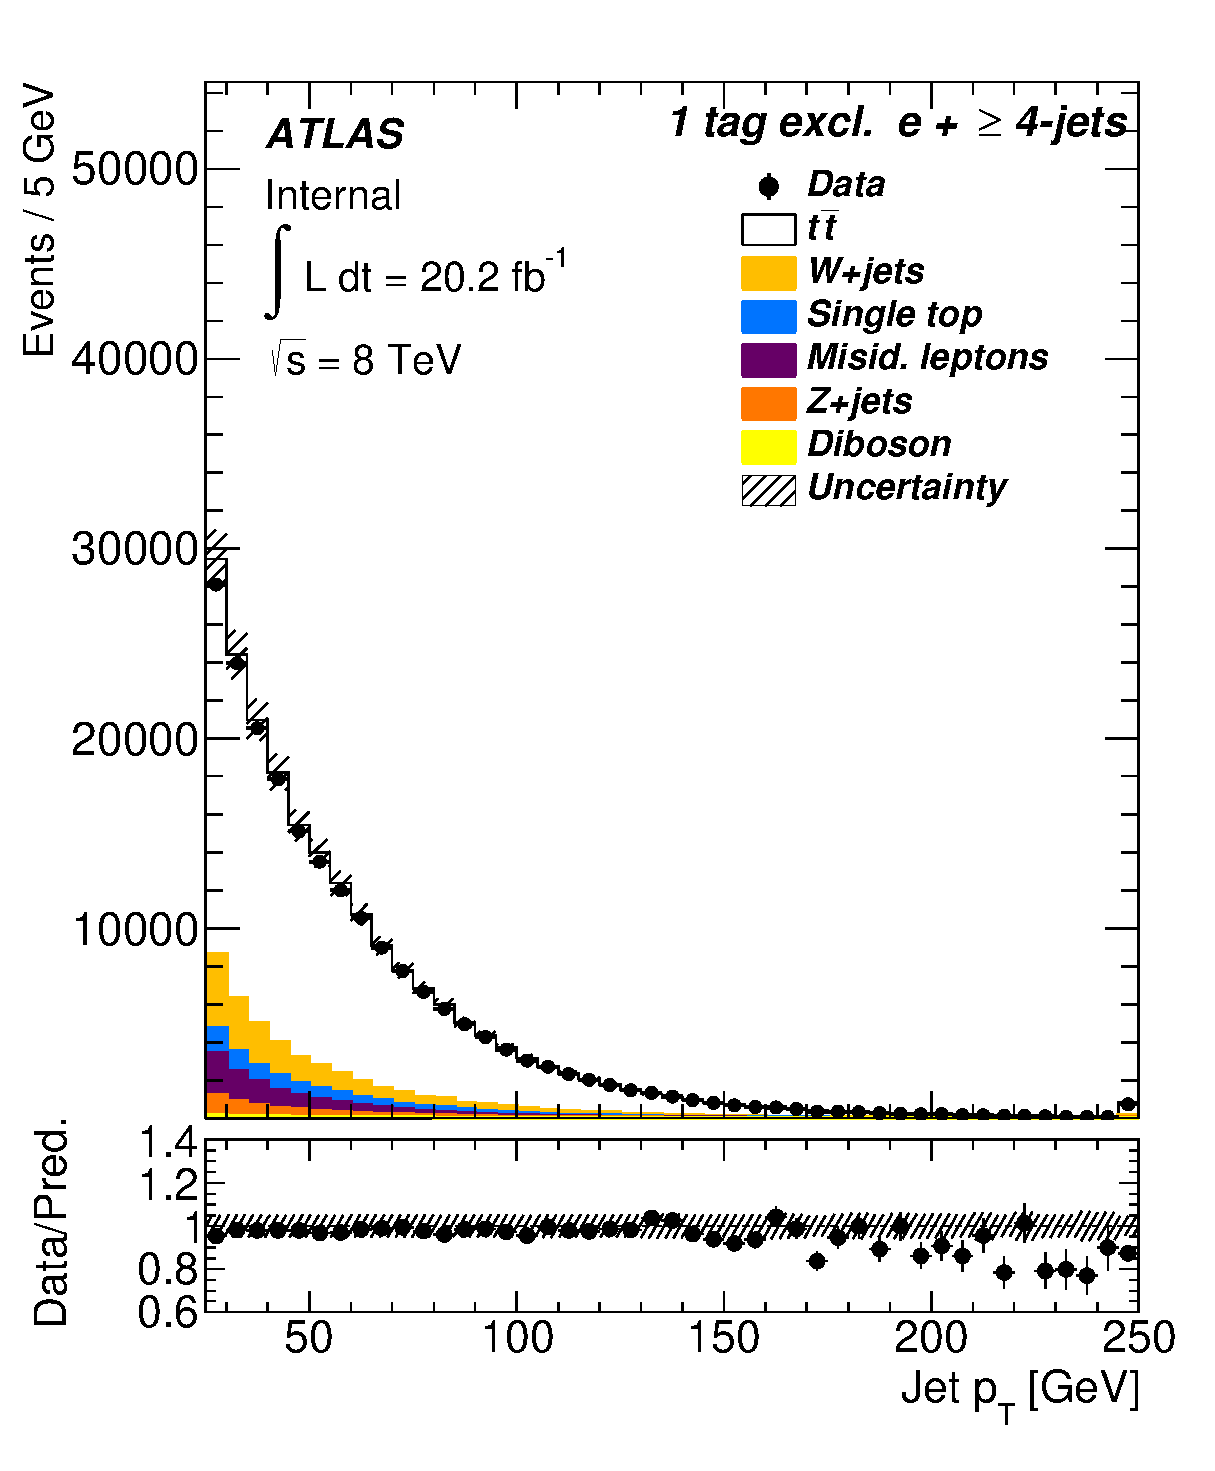
\includegraphics[height=65mm]{chapters/whel/figures/control_Plots2/bTag_1excl/JetPt_el}\\
		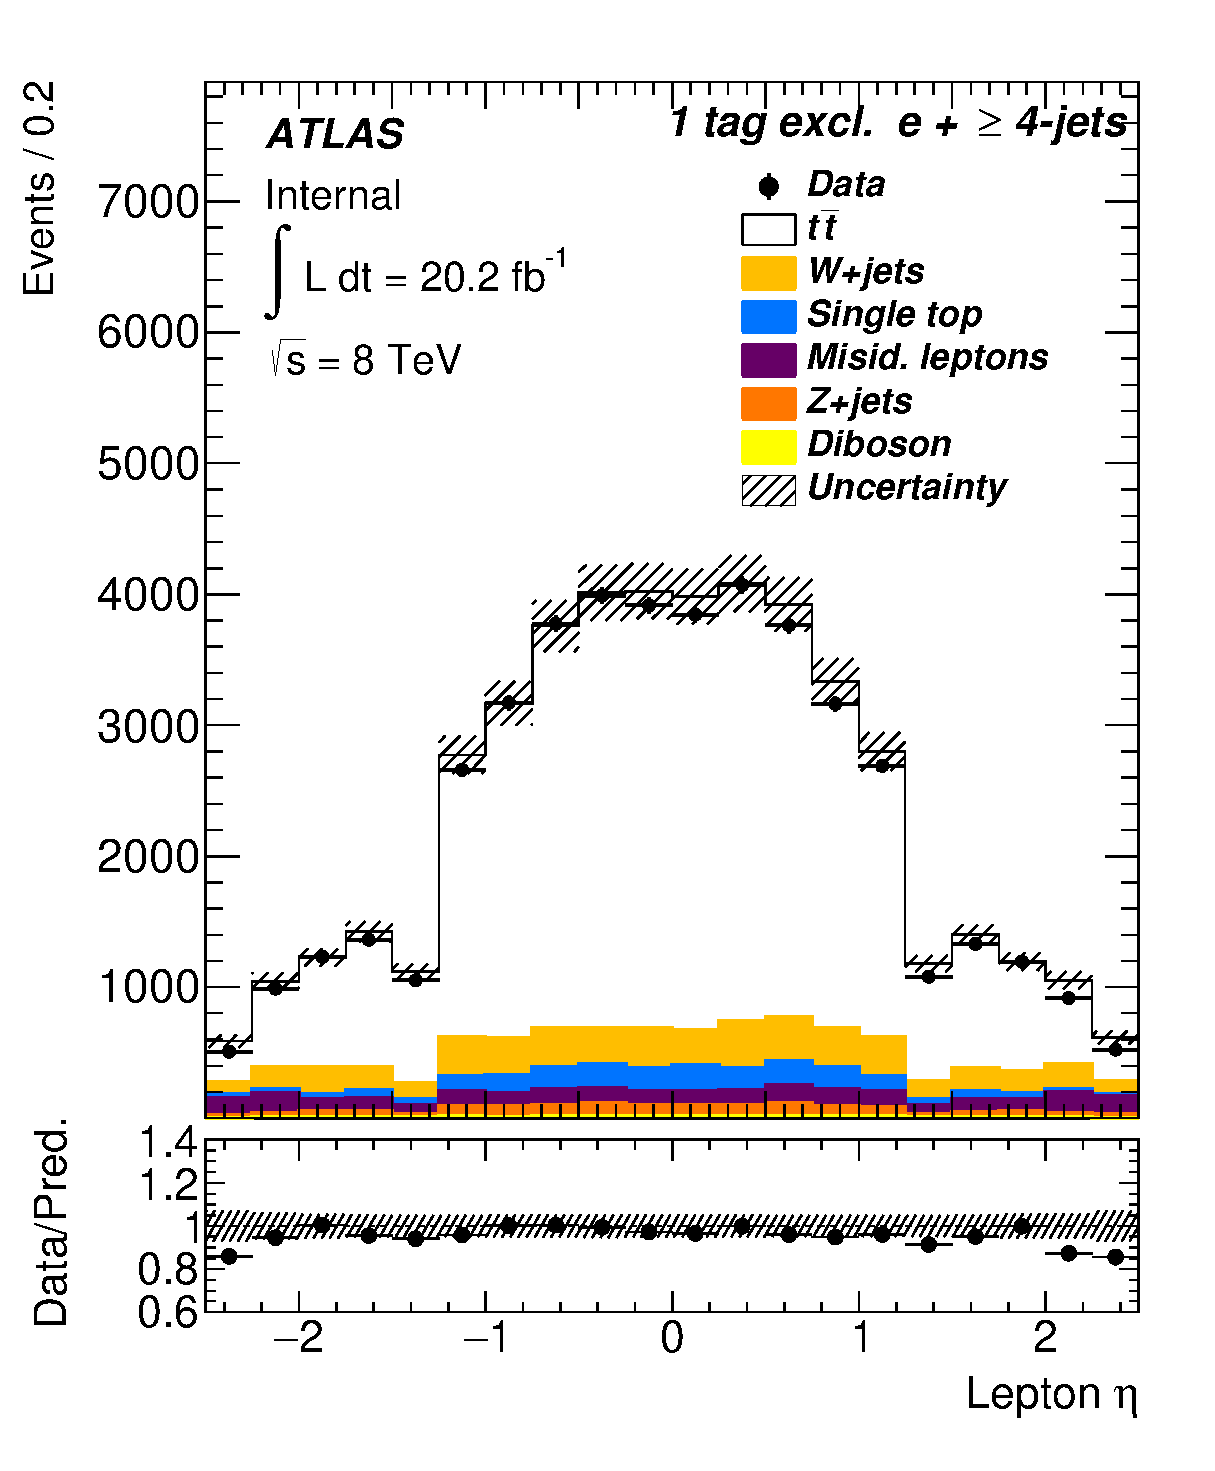
\includegraphics[height=65mm]{chapters/whel/figures/control_Plots2/bTag_1excl/LeptonEta_el}
		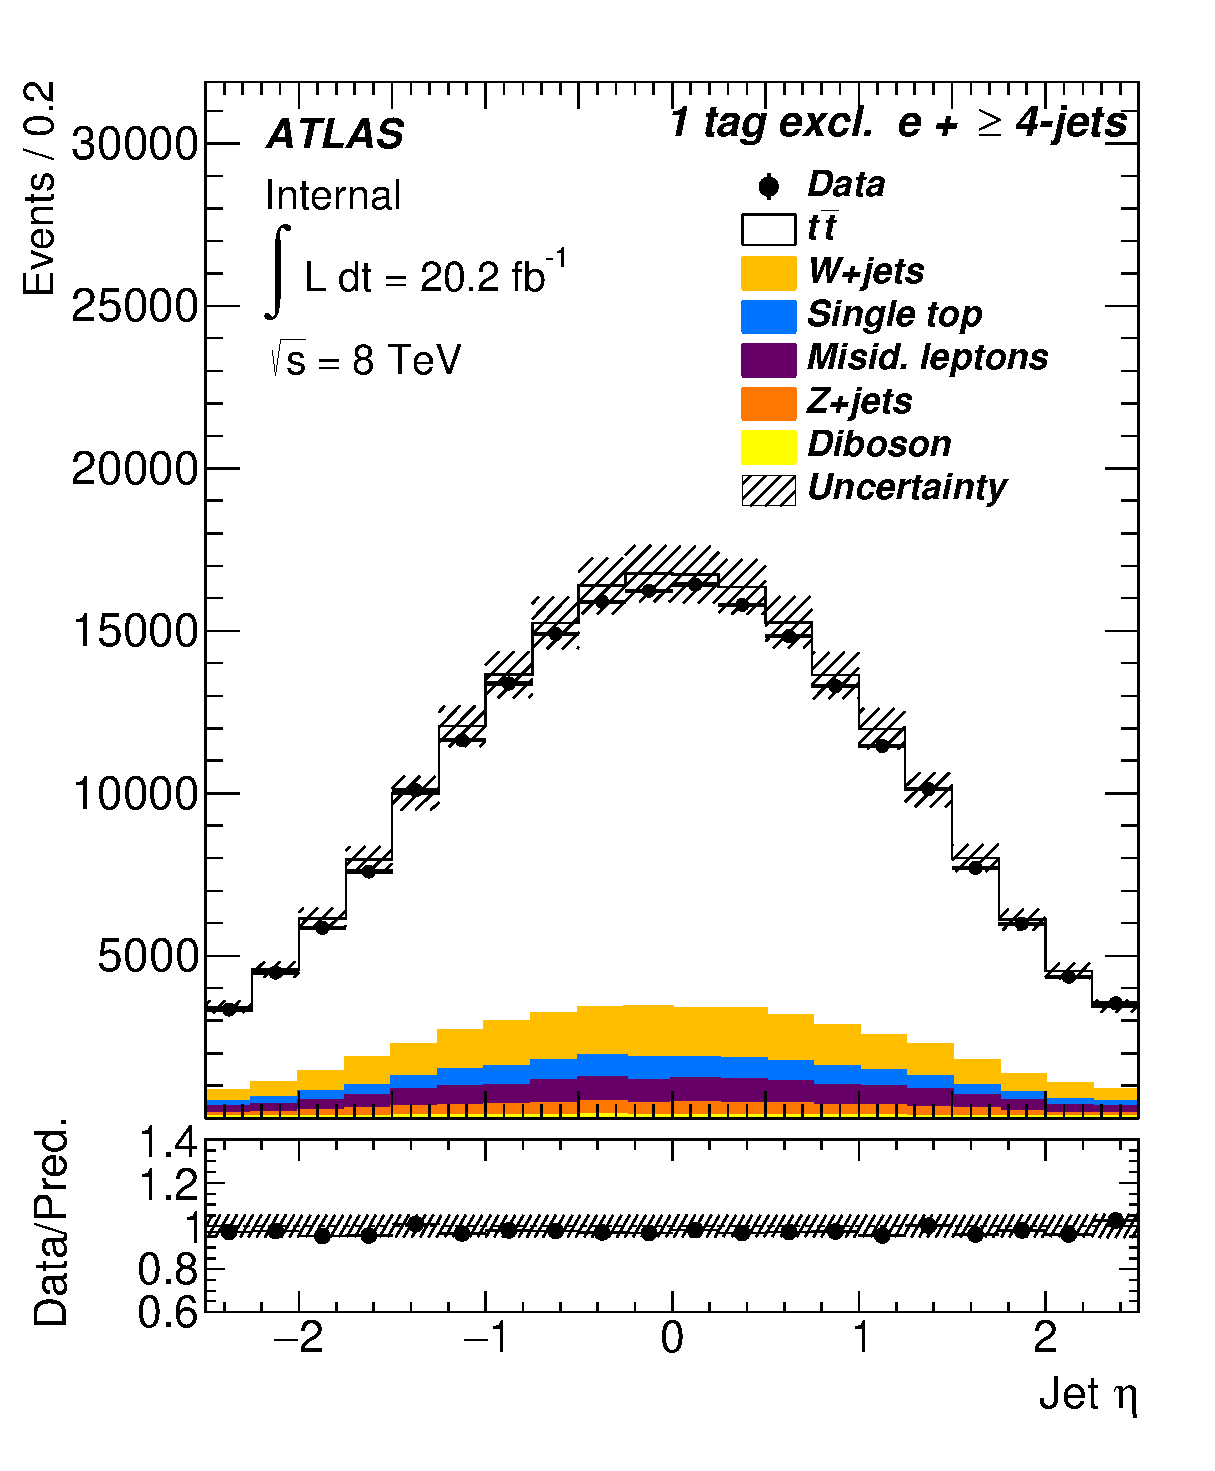
\includegraphics[height=65mm]{chapters/whel/figures/control_Plots2/bTag_1excl/JetEta_el}\\
		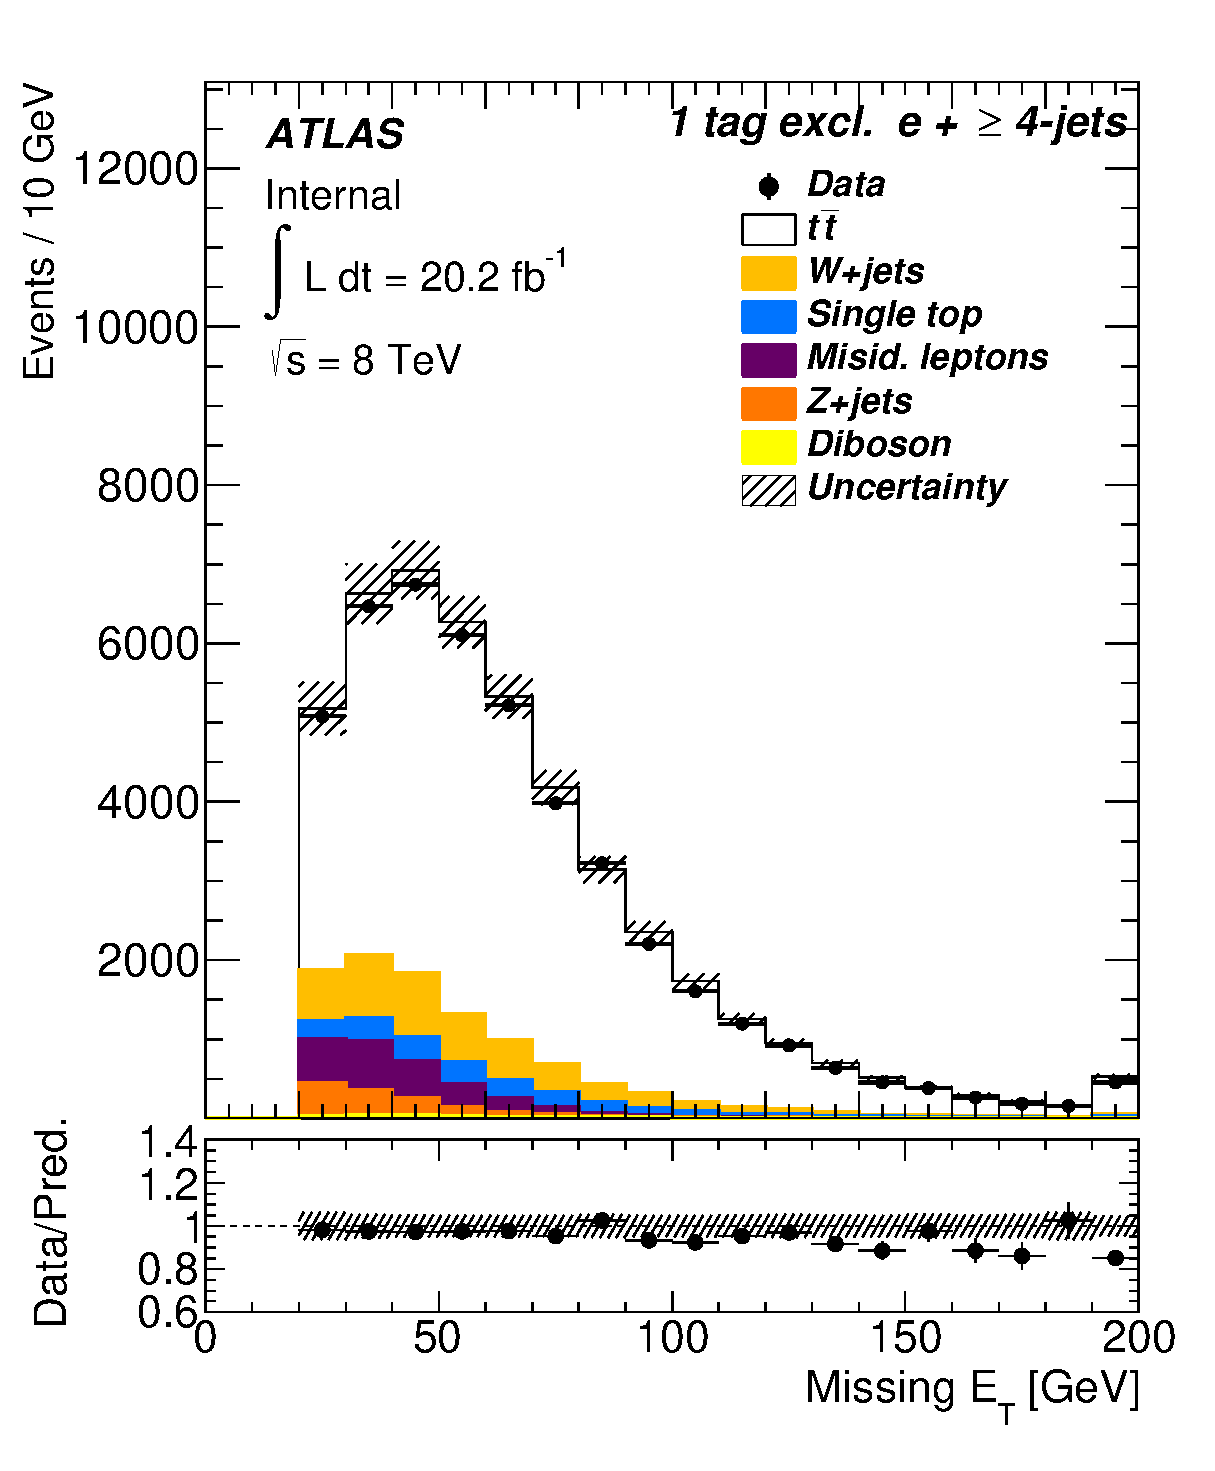
\includegraphics[height=65mm]{chapters/whel/figures/control_Plots2/bTag_1excl/MissingEt_el}
        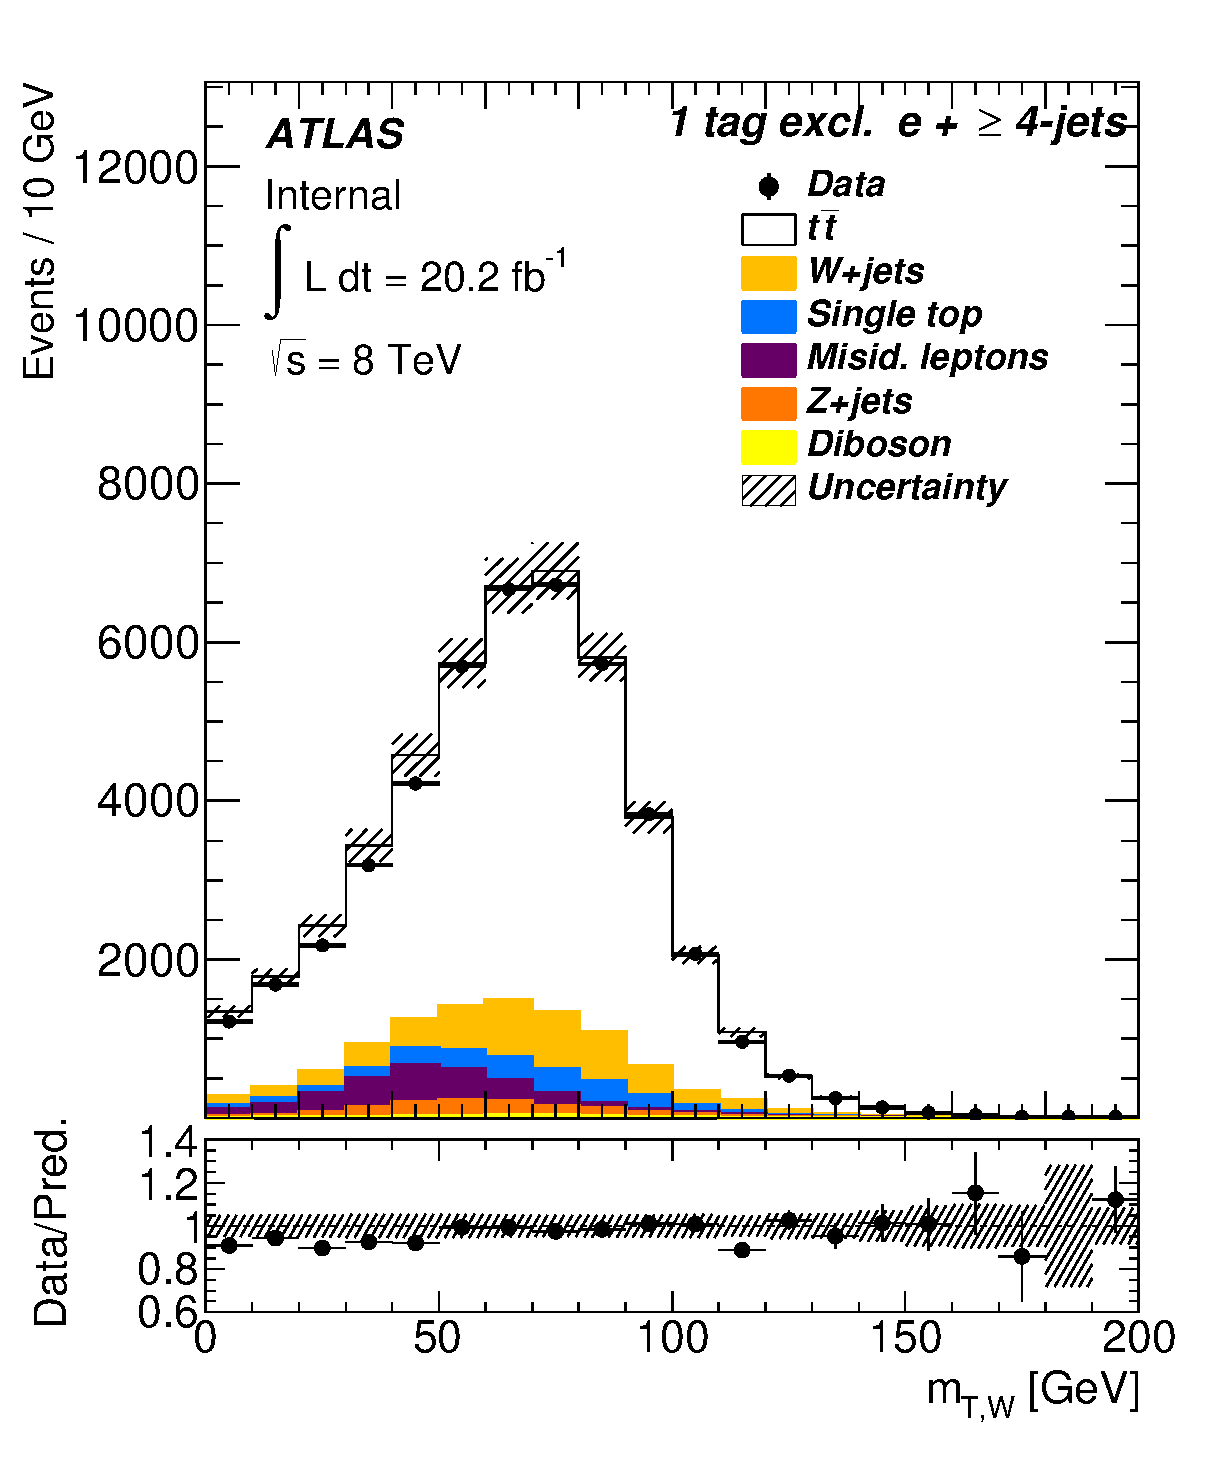
\includegraphics[height=65mm]{chapters/whel/figures/control_Plots2/bTag_1excl/TransverseMass_el}
	\caption{Plots showing data/MC agreement after event selection for reconstructed objects (lepton, jets, neutrino) in the 1 exclusive \bt tag, electron region. The shaded bands represent the Monte Carlo statistical uncertainties.}
	\label{fig:control_plots_el_1excl}
	\end{center}
	\end{figure}
	
\begin{figure}[!hb]
\begin{center}

		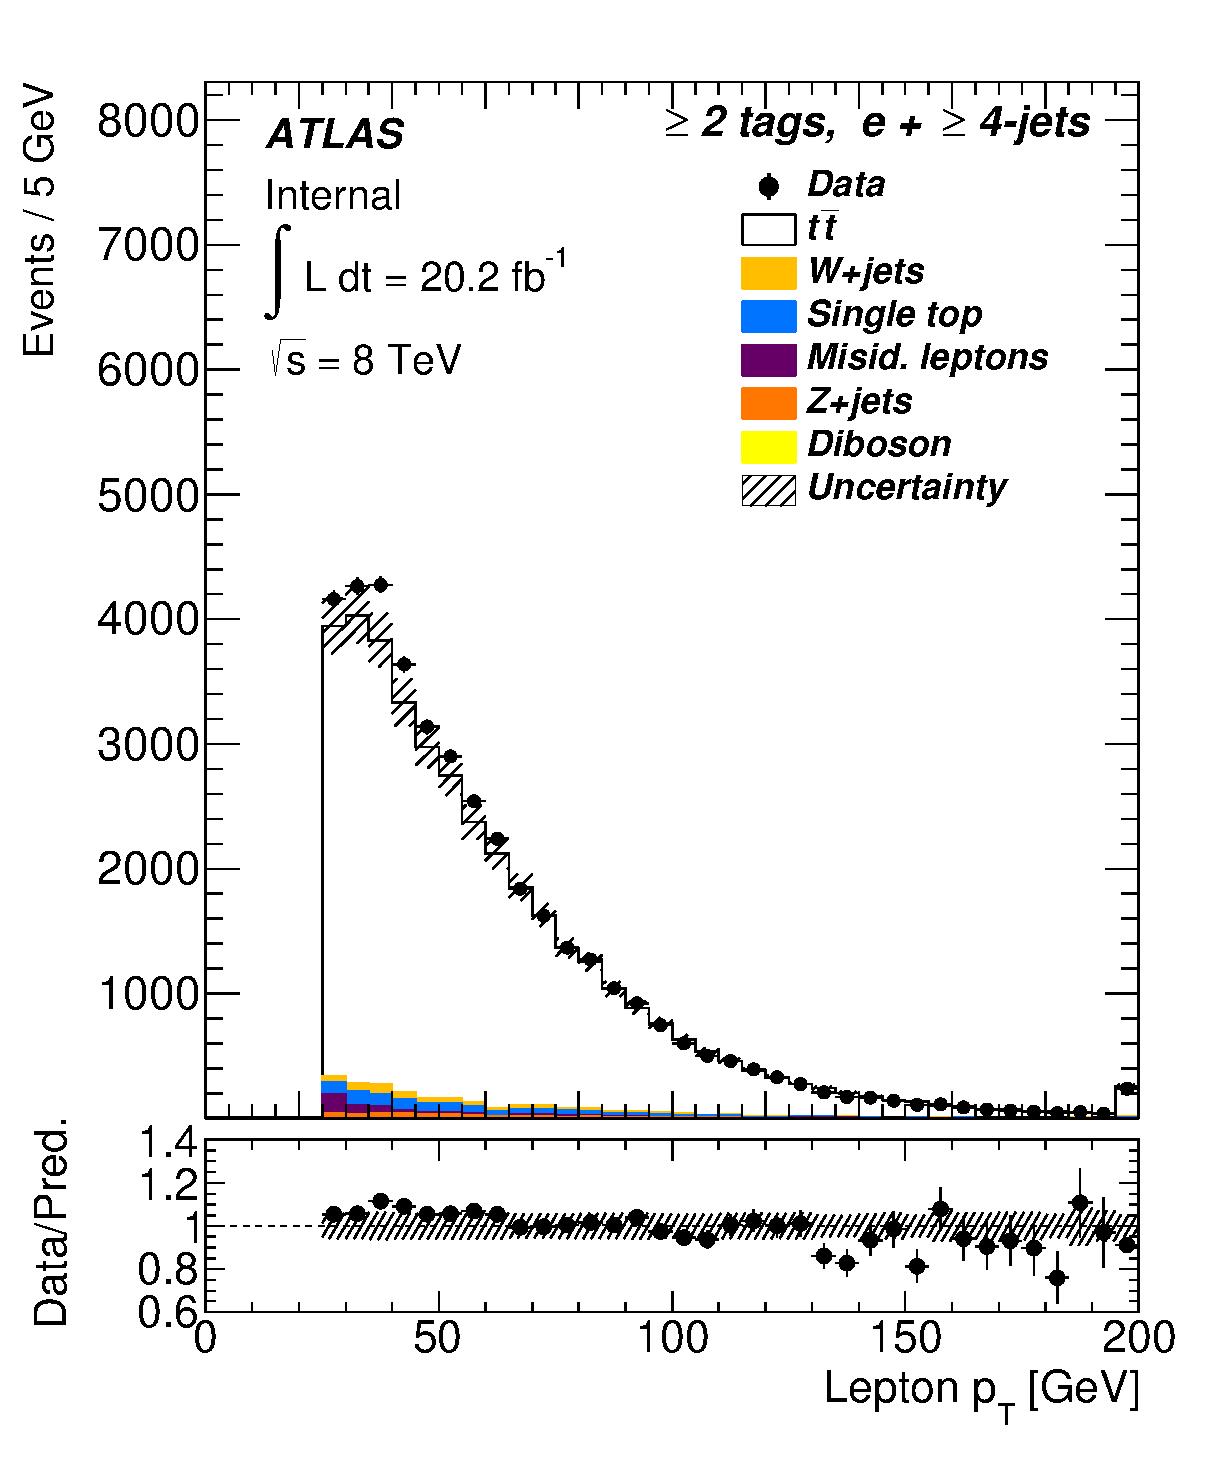
\includegraphics[height=65mm]{chapters/whel/figures/control_Plots2/bTag_2incl/LeptonPt_el}
		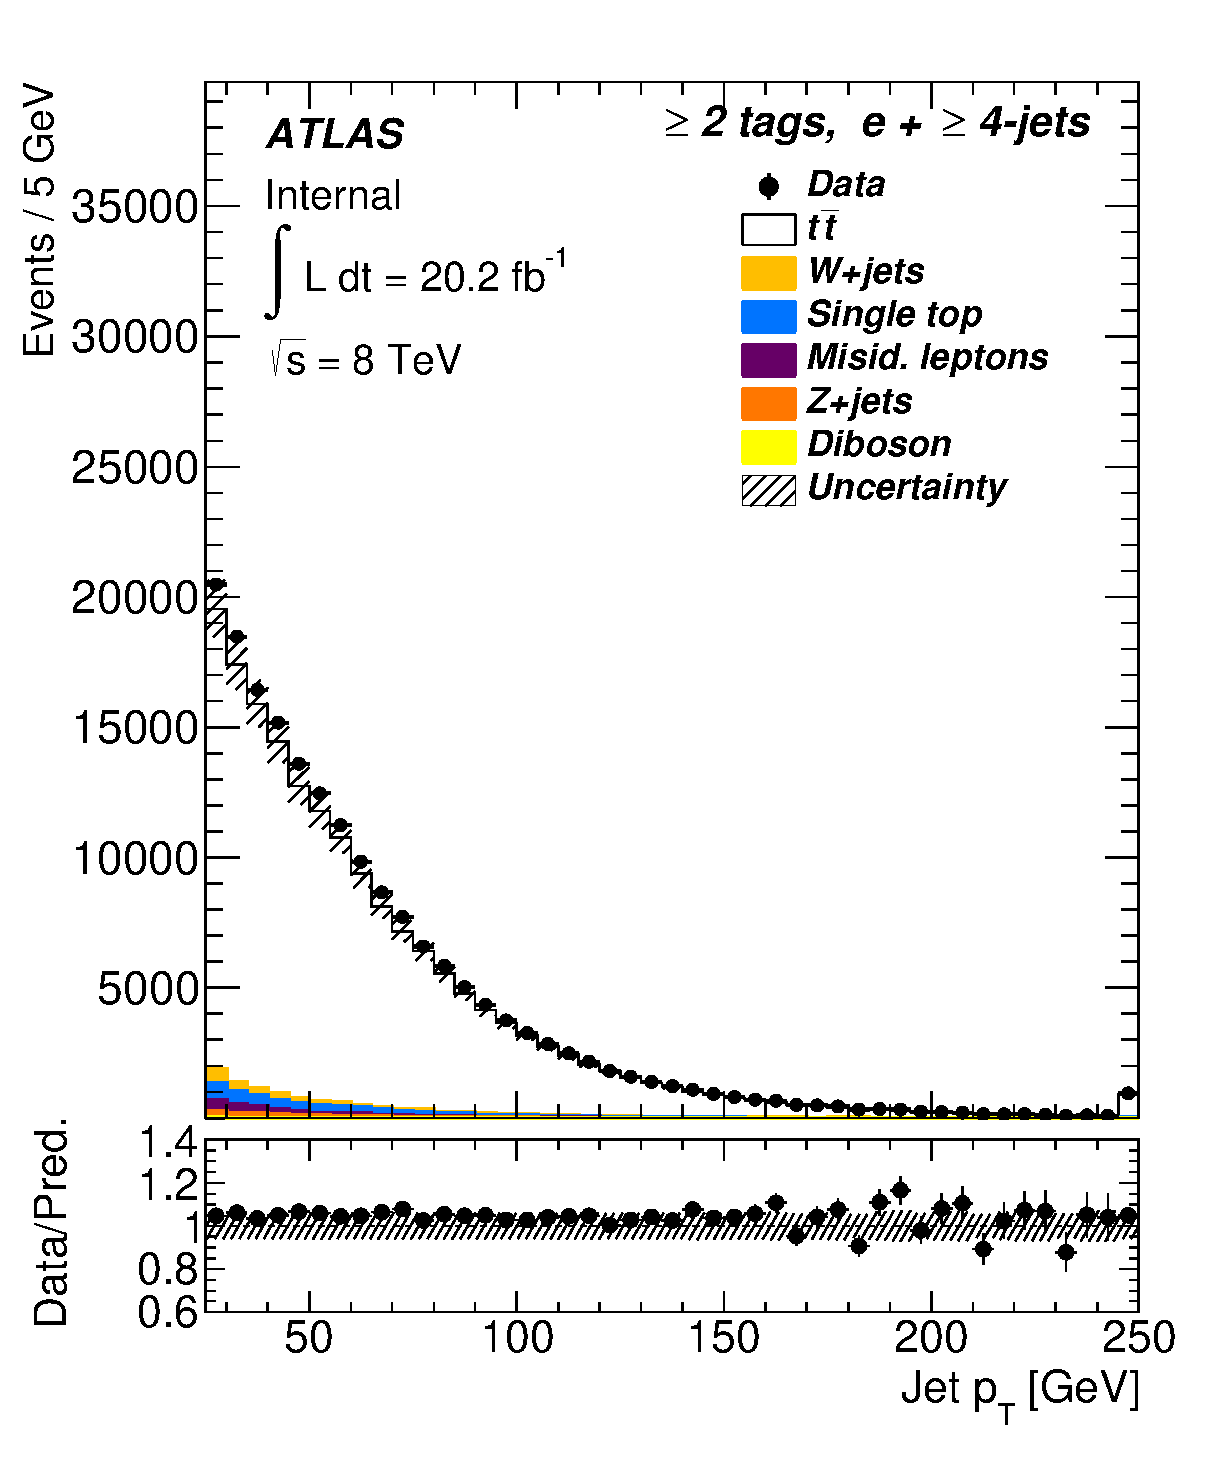
\includegraphics[height=65mm]{chapters/whel/figures/control_Plots2/bTag_2incl/JetPt_el}\\
		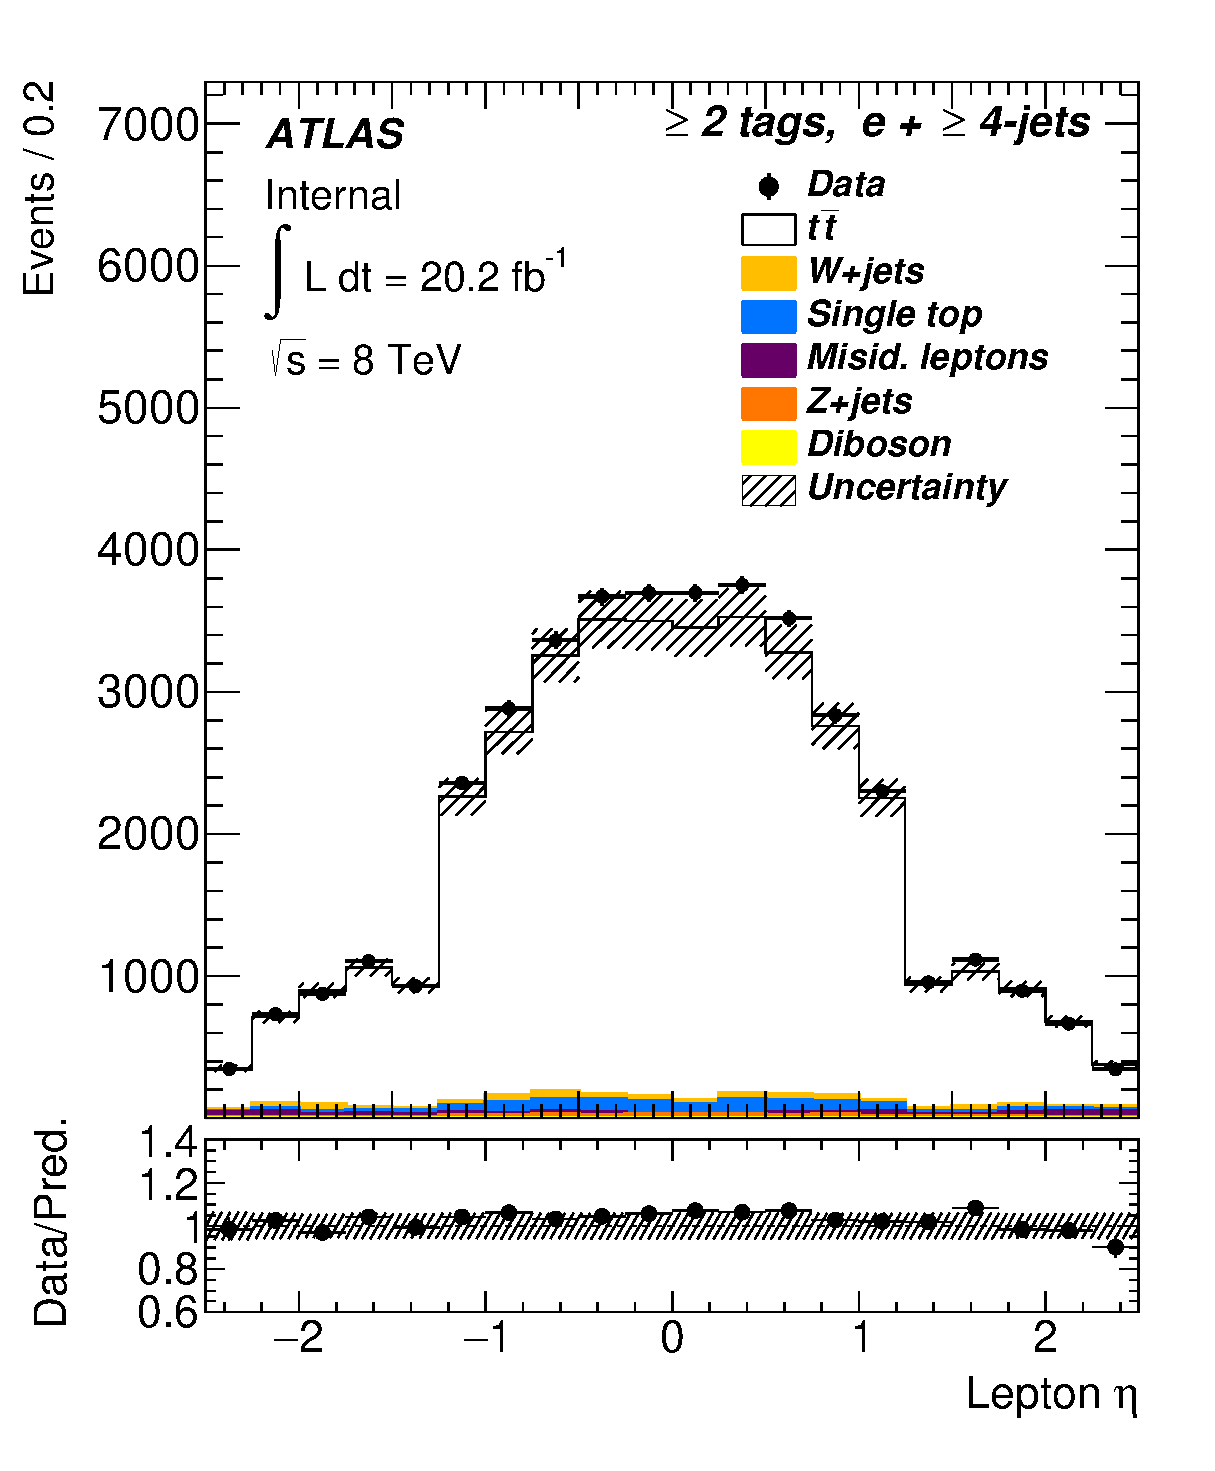
\includegraphics[height=65mm]{chapters/whel/figures/control_Plots2/bTag_2incl/LeptonEta_el}
		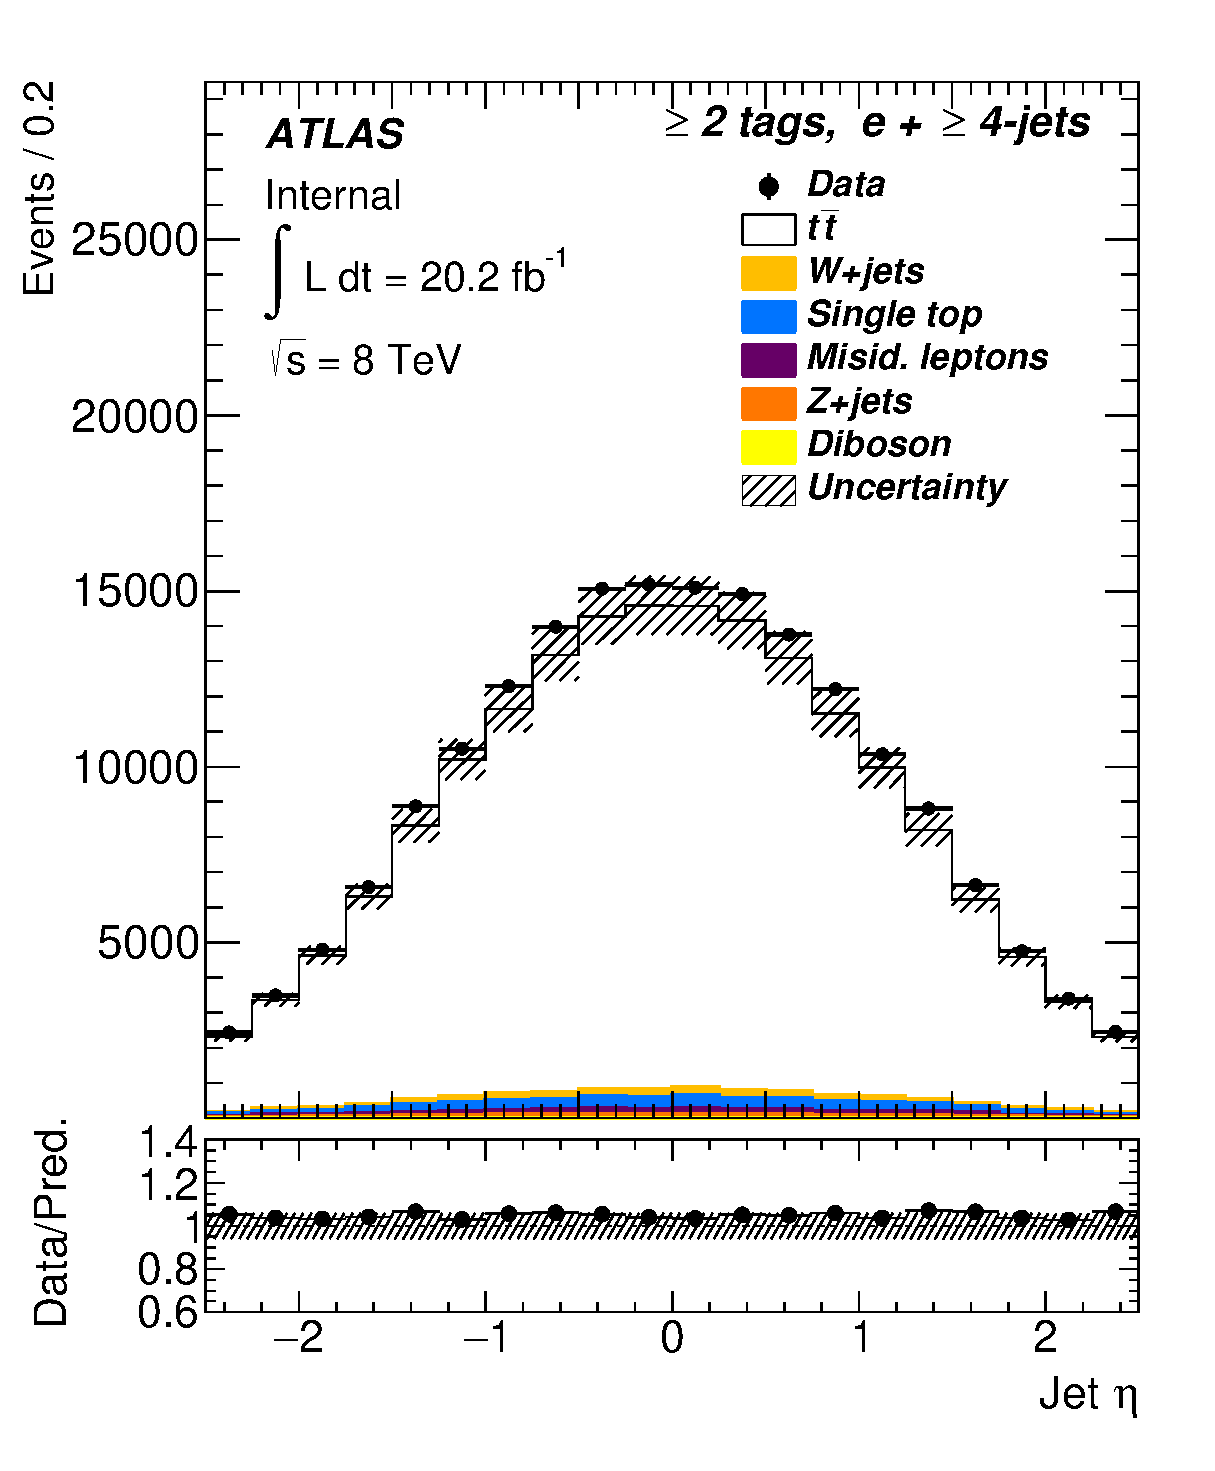
\includegraphics[height=65mm]{chapters/whel/figures/control_Plots2/bTag_2incl/JetEta_el}\\
		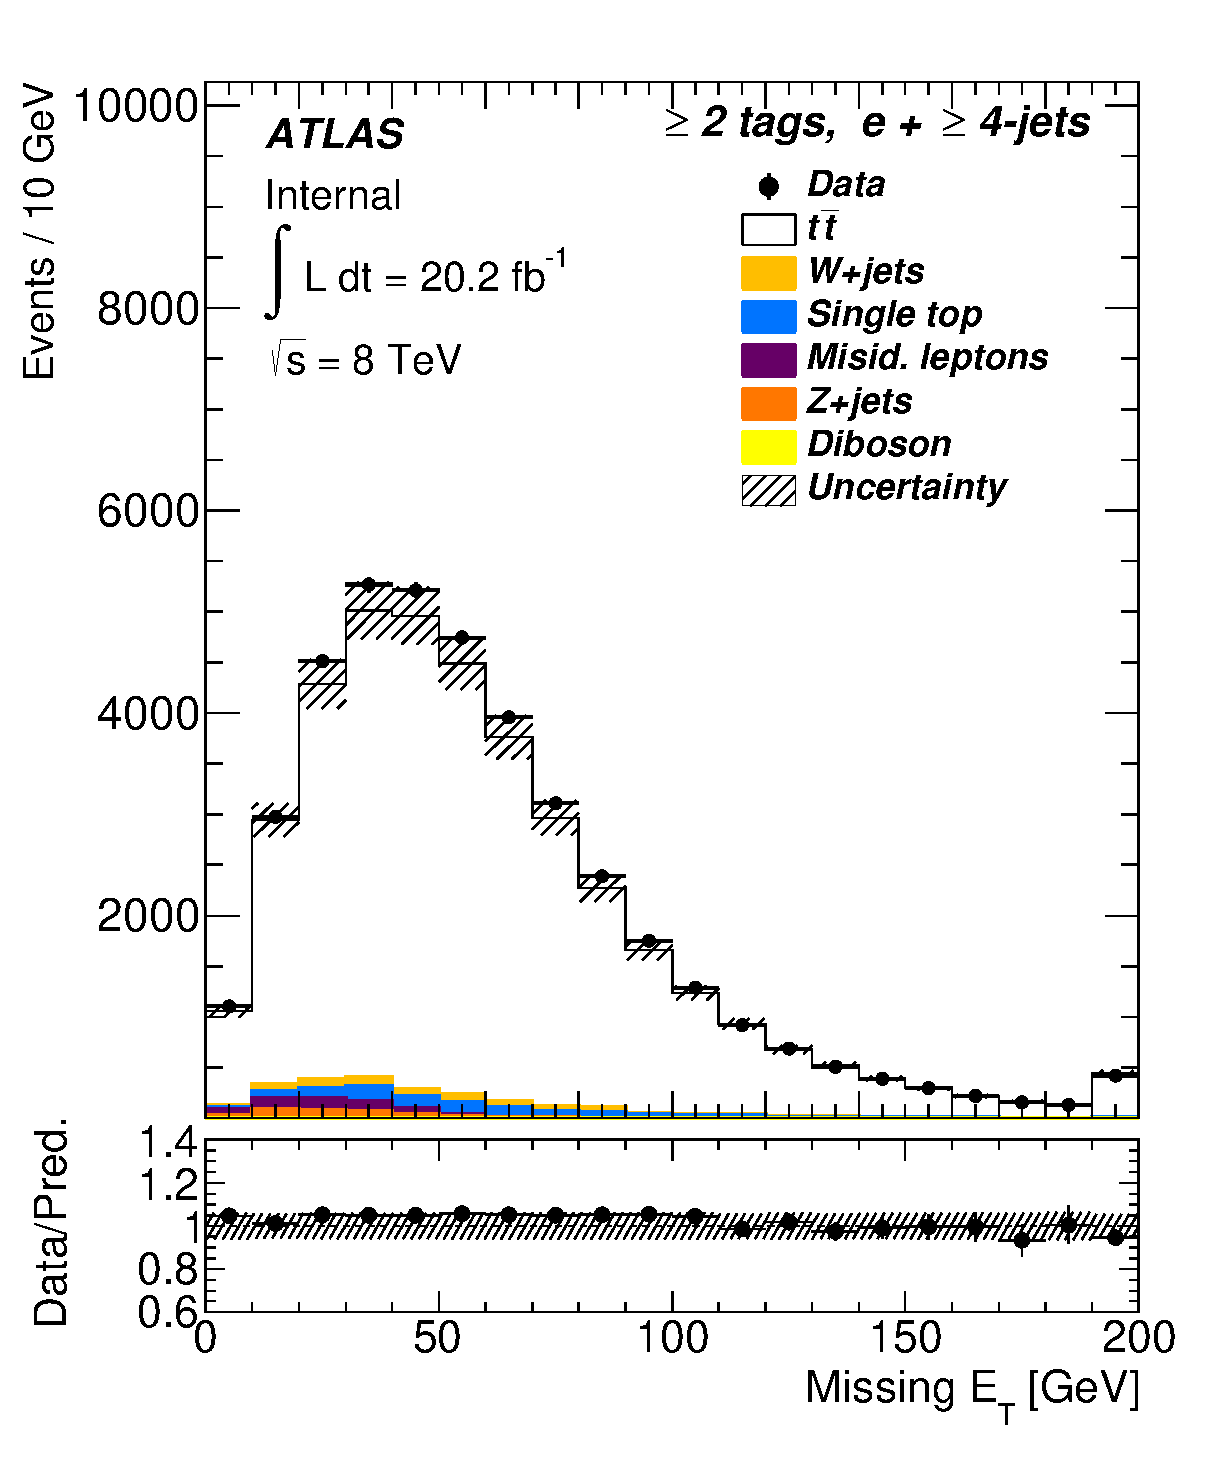
\includegraphics[height=65mm]{chapters/whel/figures/control_Plots2/bTag_2incl/MissingEt_el}
        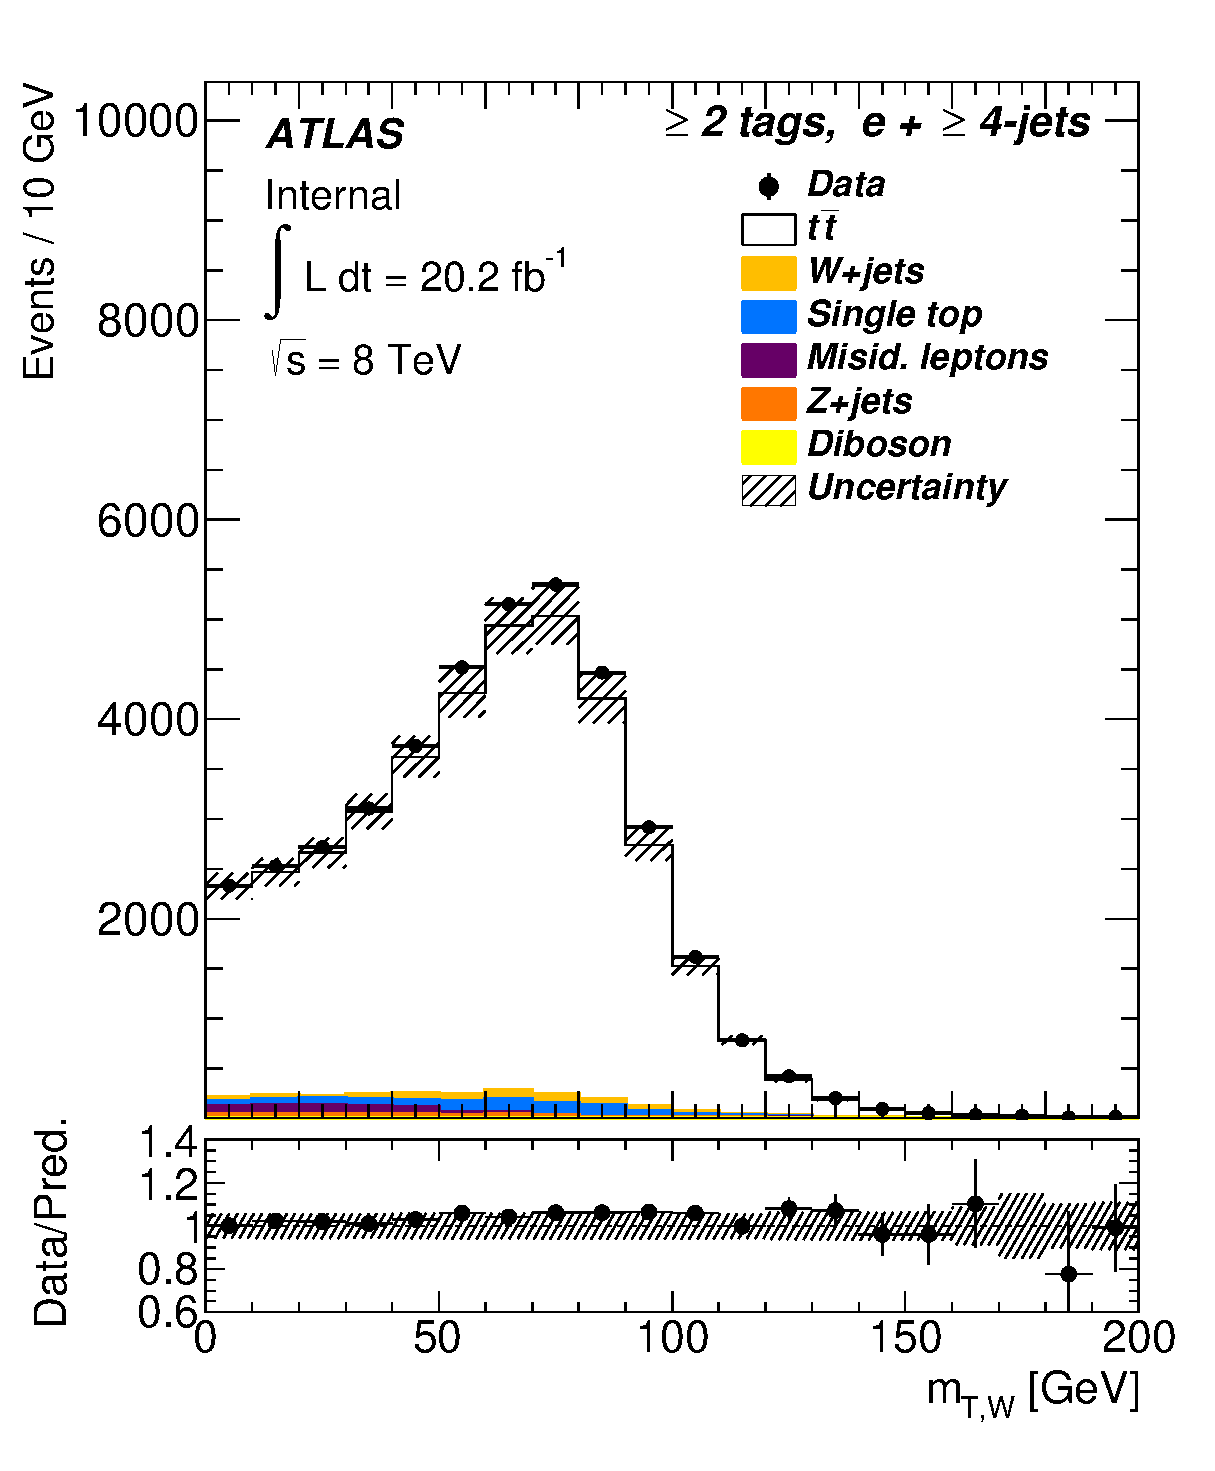
\includegraphics[height=65mm]{chapters/whel/figures/control_Plots2/bTag_2incl/TransverseMass_el}
	\caption{Plots showing data/MC agreement after event selection for reconstructed objects (lepton, jets, neutrino) in the 2 inclusive \bt tag, electron region. The shaded bands represent the Monte Carlo statistical uncertainties.}
	\label{fig:control_plots_el_2incl}
	\end{center}
	\end{figure}
	

\begin{figure}[!hb]
\begin{center}

		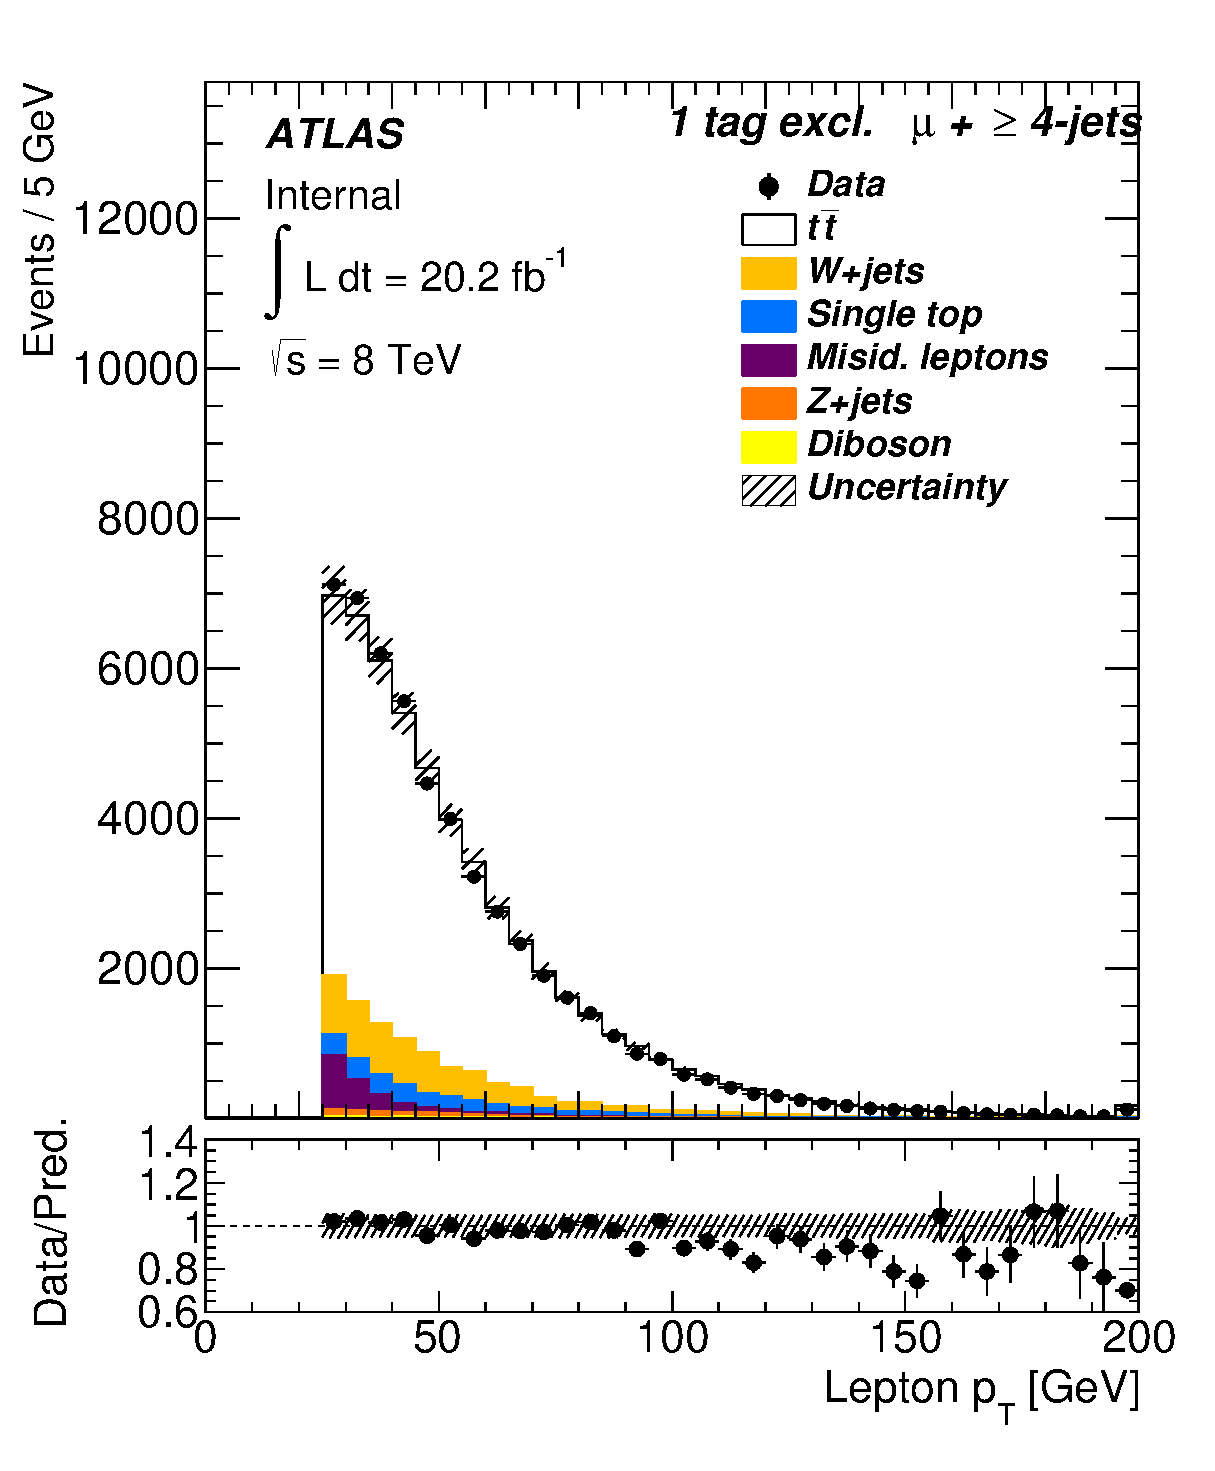
\includegraphics[height=65mm]{chapters/whel/figures/control_Plots2/bTag_1excl/LeptonPt_mu}
		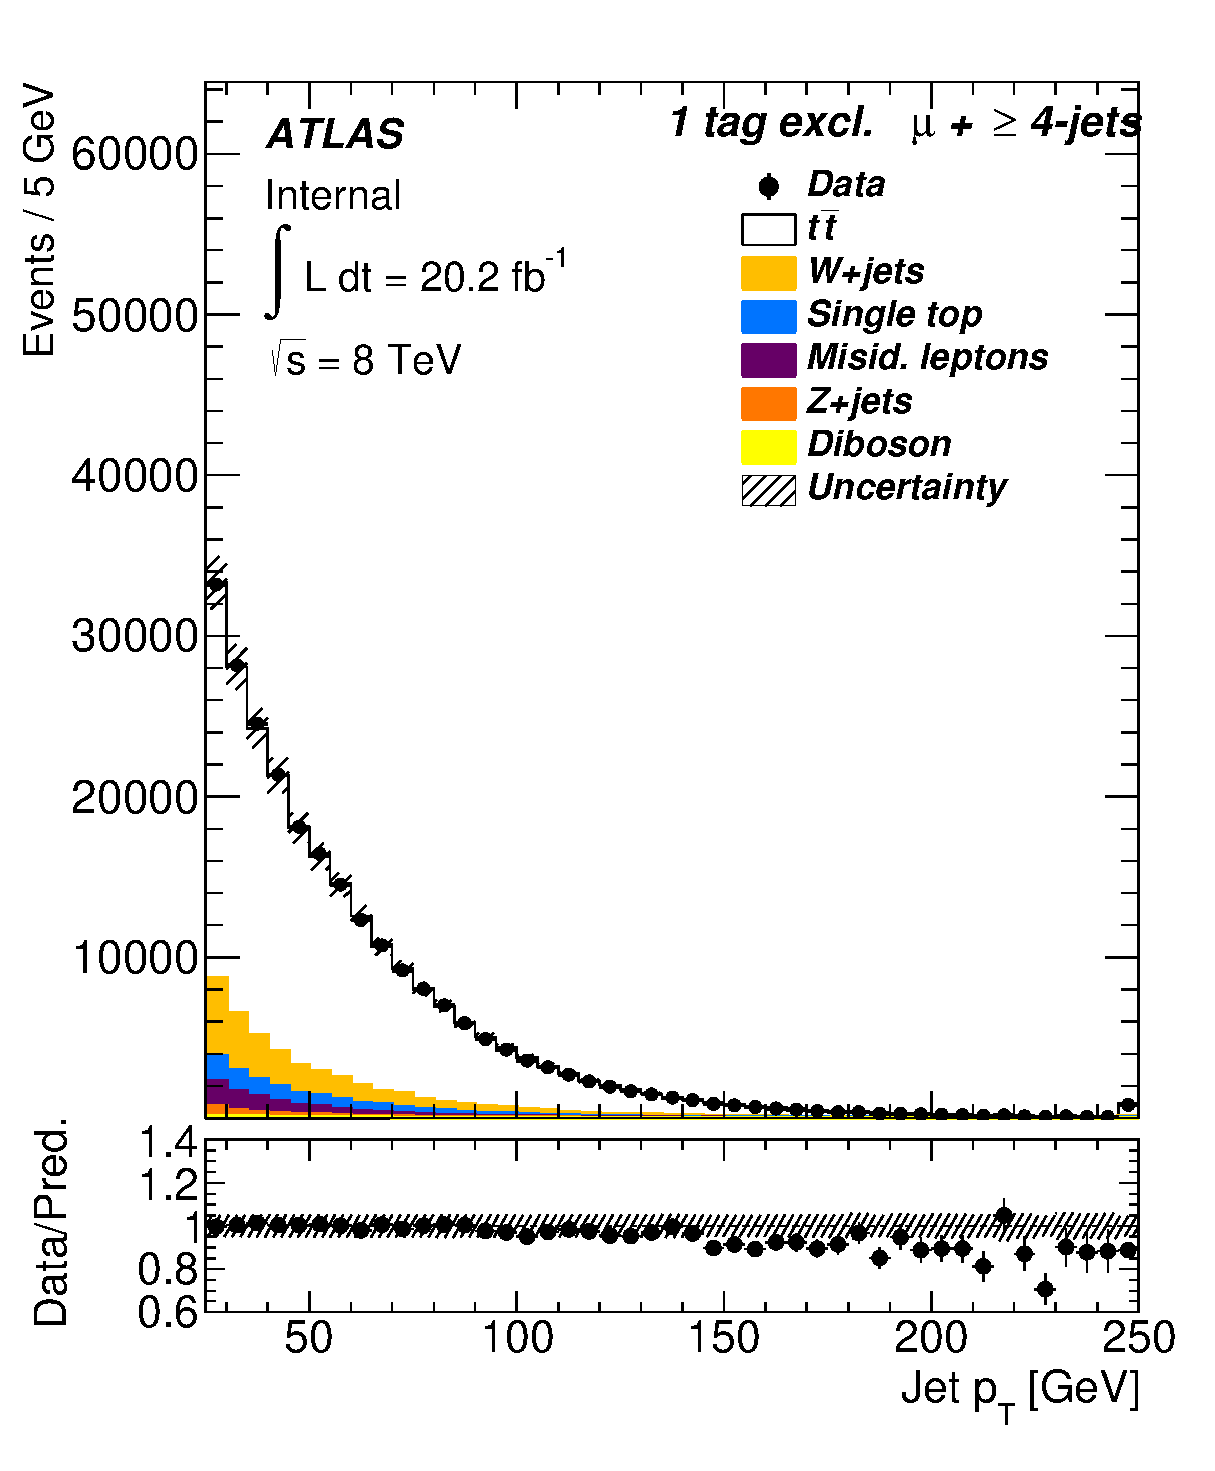
\includegraphics[height=65mm]{chapters/whel/figures/control_Plots2/bTag_1excl/JetPt_mu}\\
		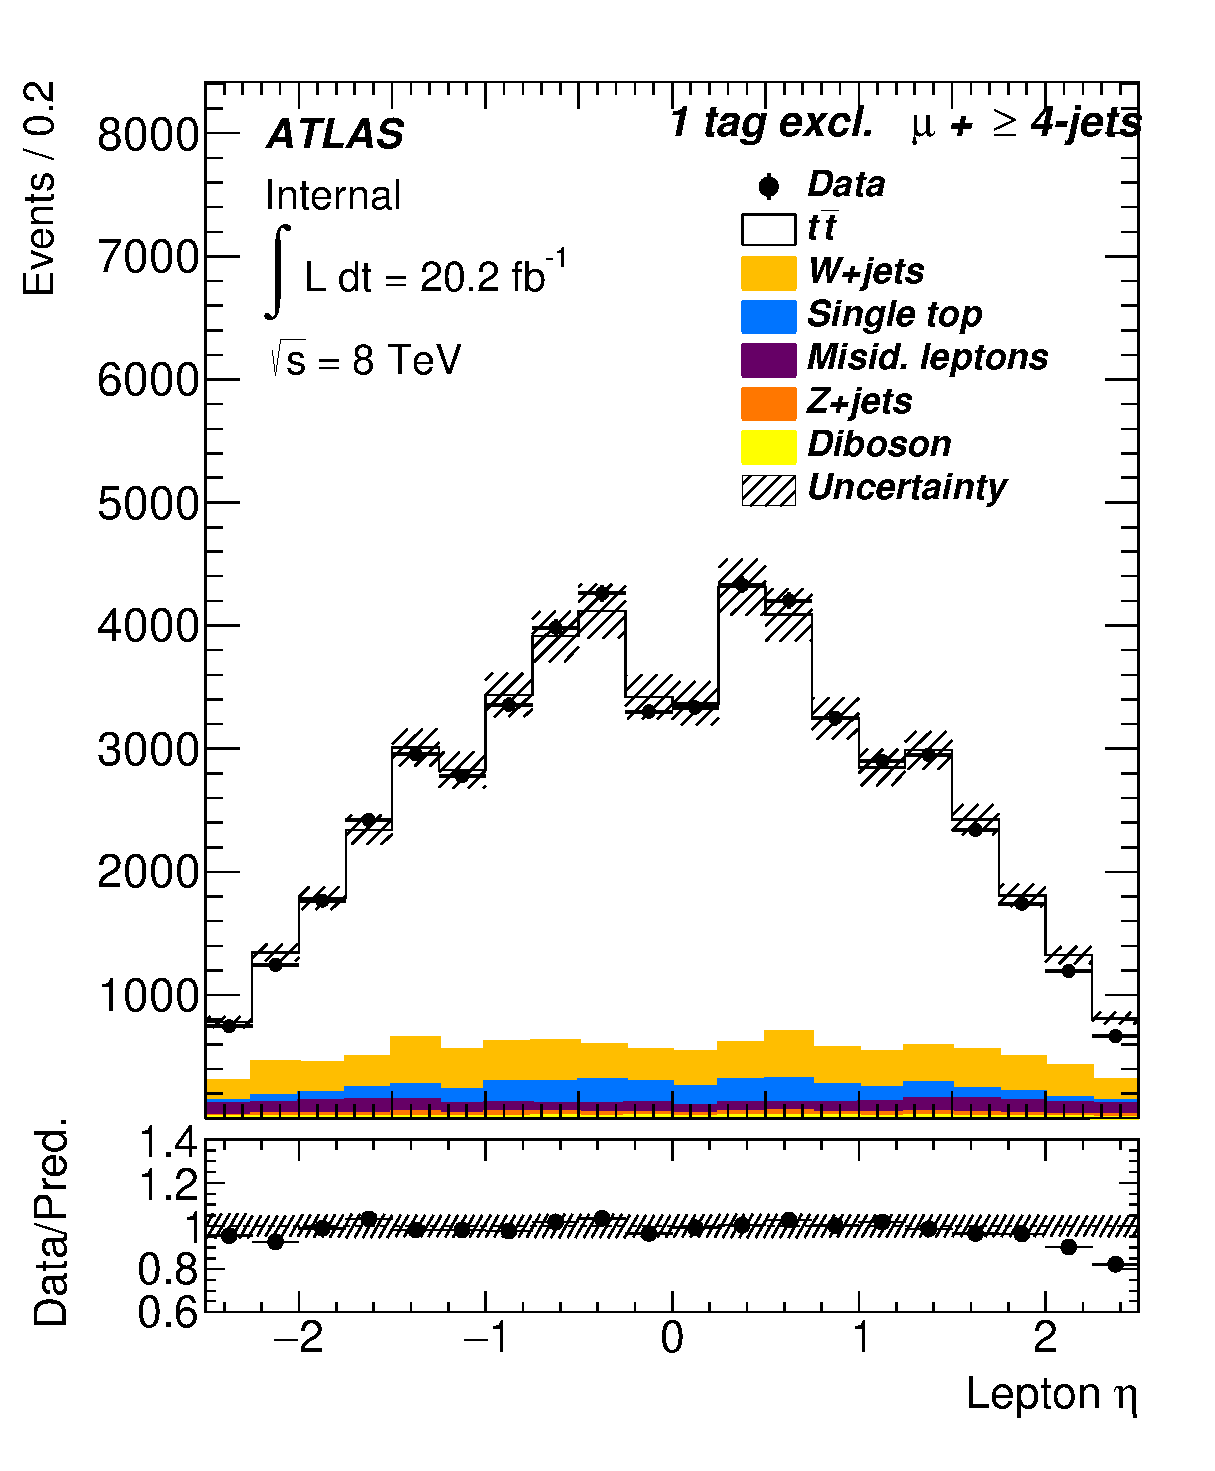
\includegraphics[height=65mm]{chapters/whel/figures/control_Plots2/bTag_1excl/LeptonEta_mu}
		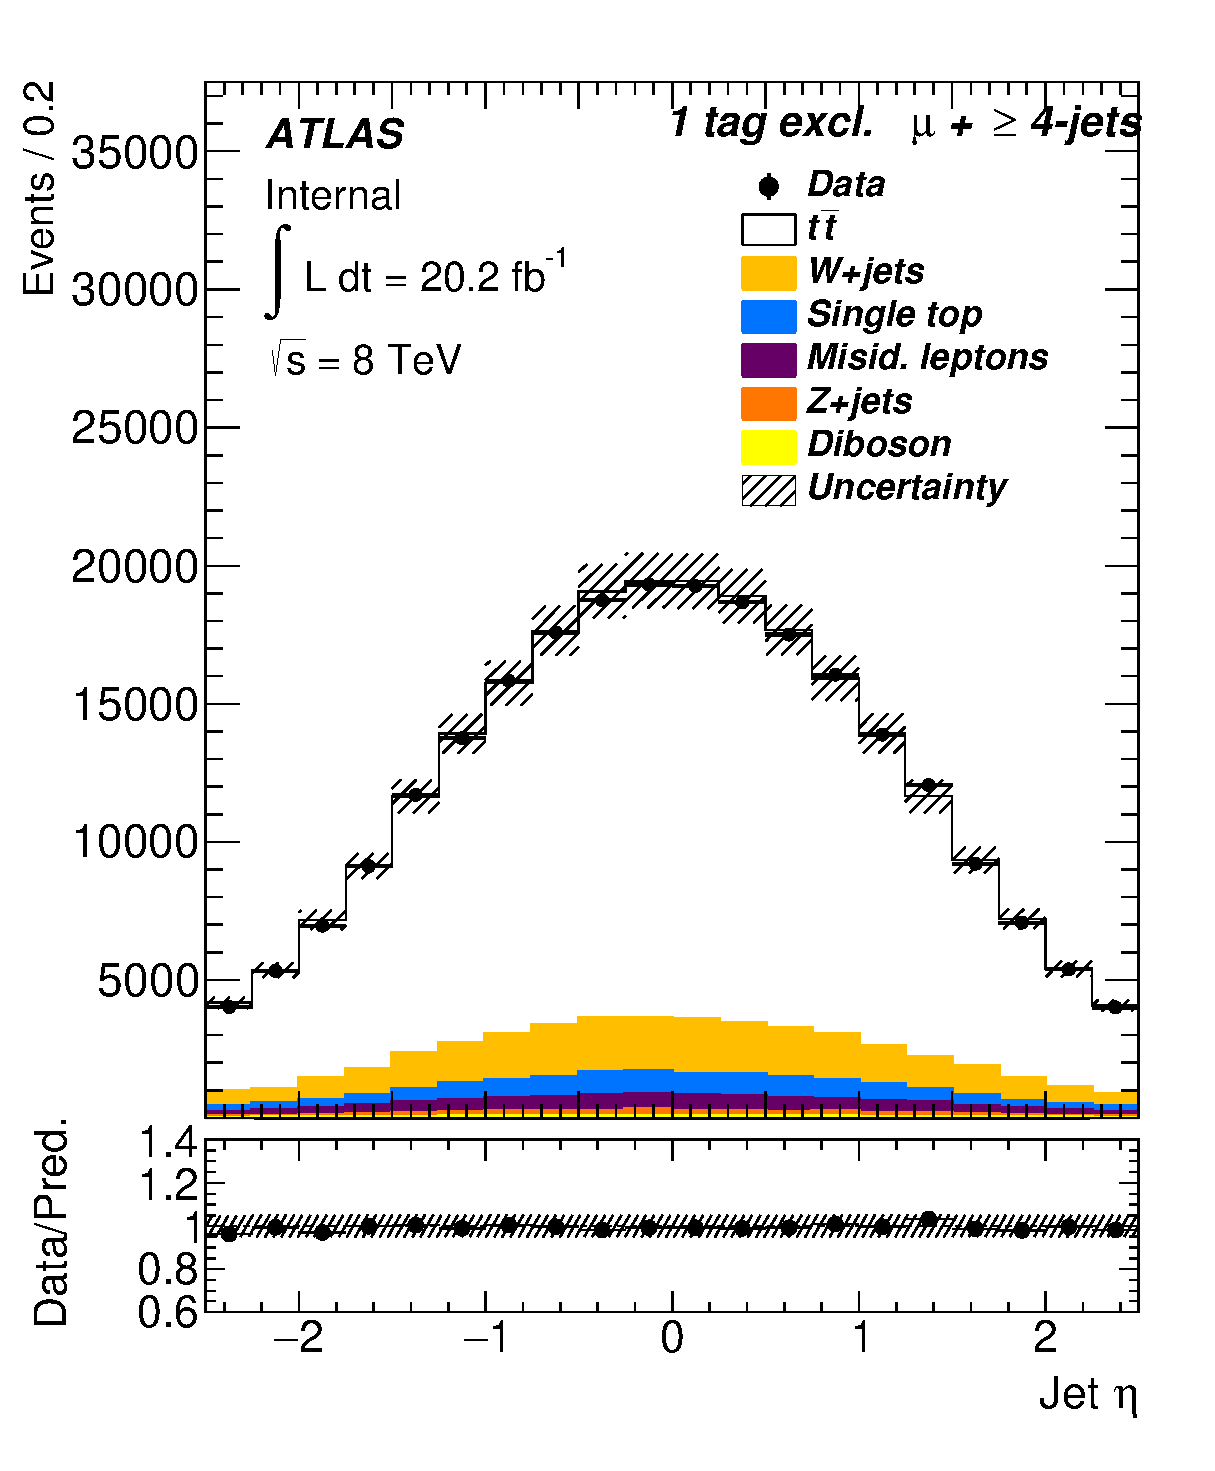
\includegraphics[height=65mm]{chapters/whel/figures/control_Plots2/bTag_1excl/JetEta_mu}\\
		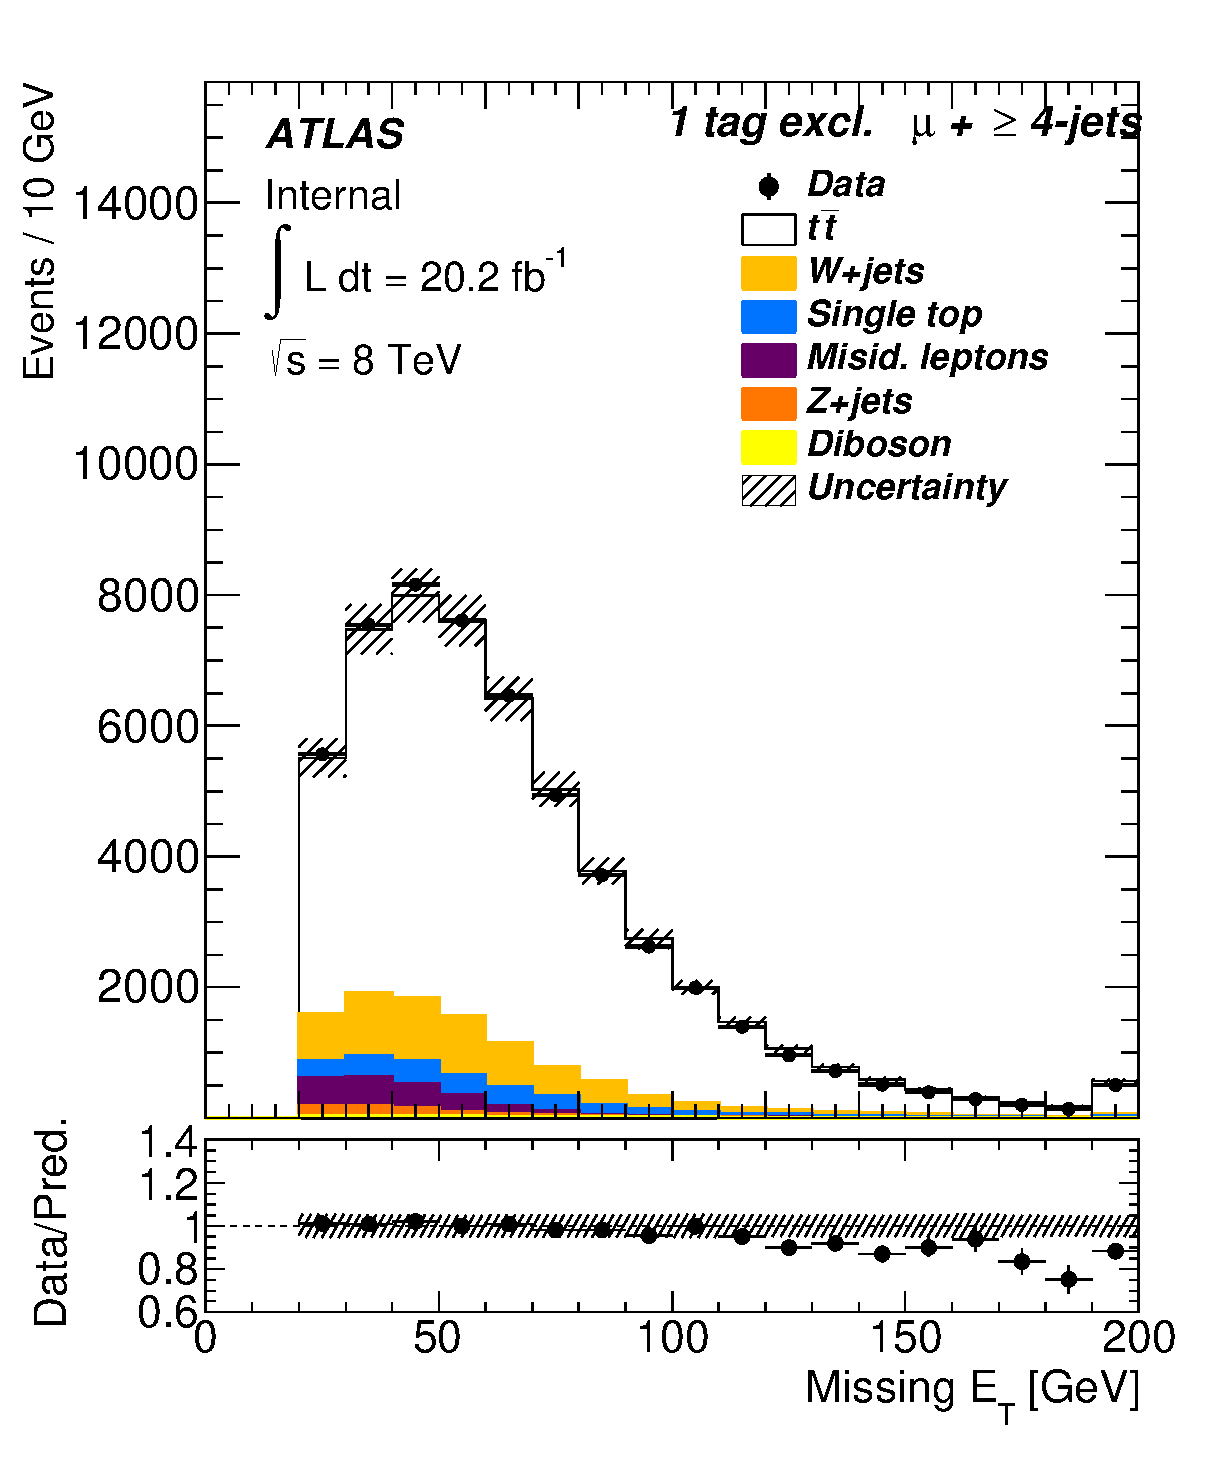
\includegraphics[height=65mm]{chapters/whel/figures/control_Plots2/bTag_1excl/MissingEt_mu}
        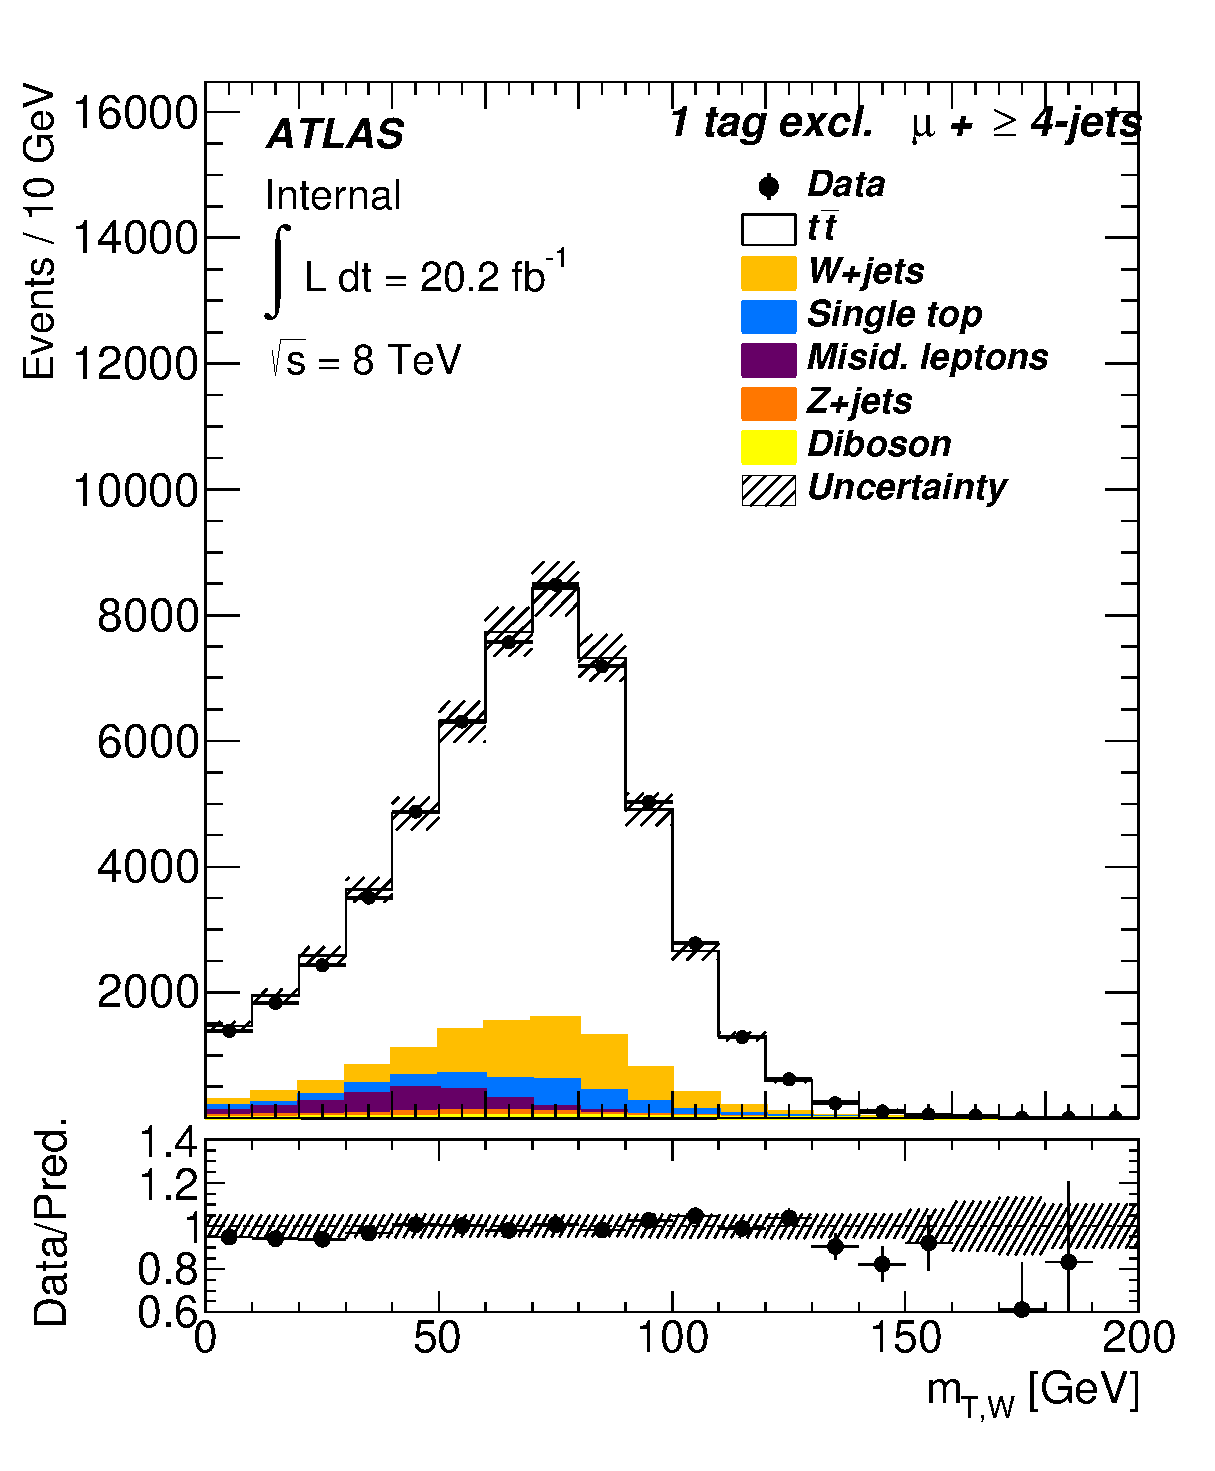
\includegraphics[height=65mm]{chapters/whel/figures/control_Plots2/bTag_1excl/TransverseMass_mu}
	\caption{Plots showing data/MC agreement after event selection for reconstructed objects (lepton, jets, neutrino) in the 1 exclusive \bt tag, muon region. The shaded bands represent the Monte Carlo statistical uncertainties.}
	\label{fig:control_plots_mu_1excl}
	\end{center}
	\end{figure}
	
\begin{figure}[!hb]
\begin{center}

		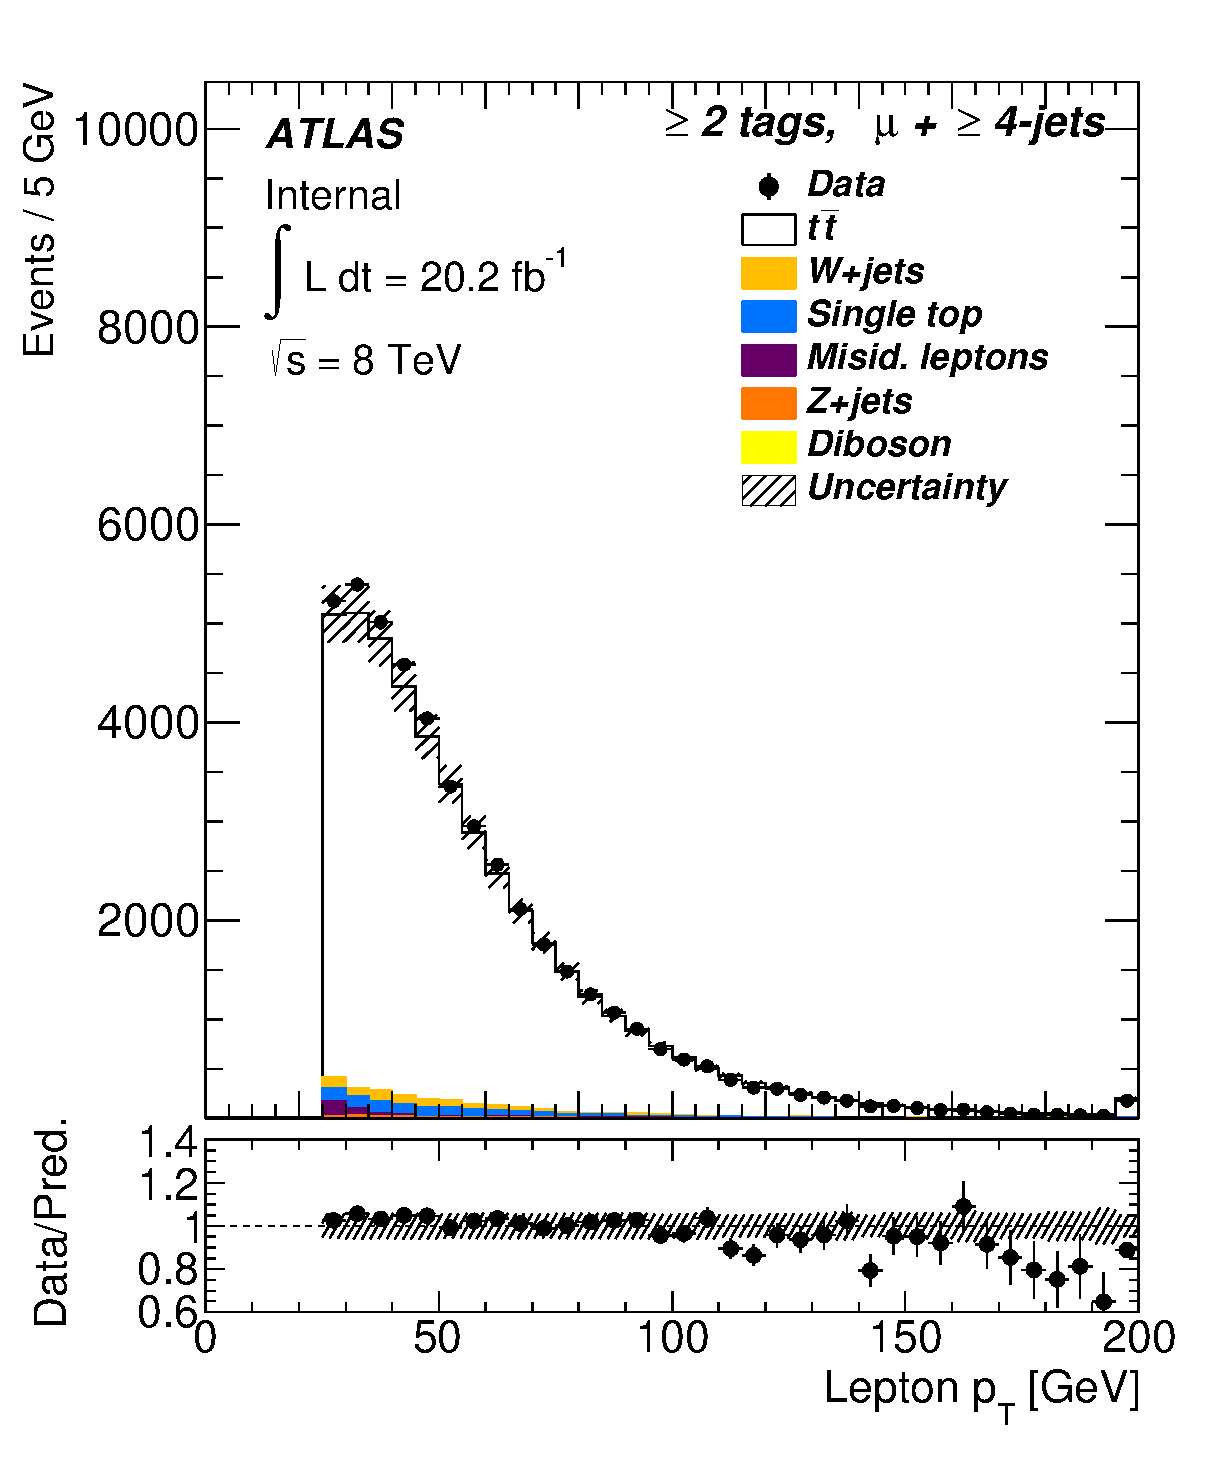
\includegraphics[height=65mm]{chapters/whel/figures/control_Plots2/bTag_2incl/LeptonPt_mu}
		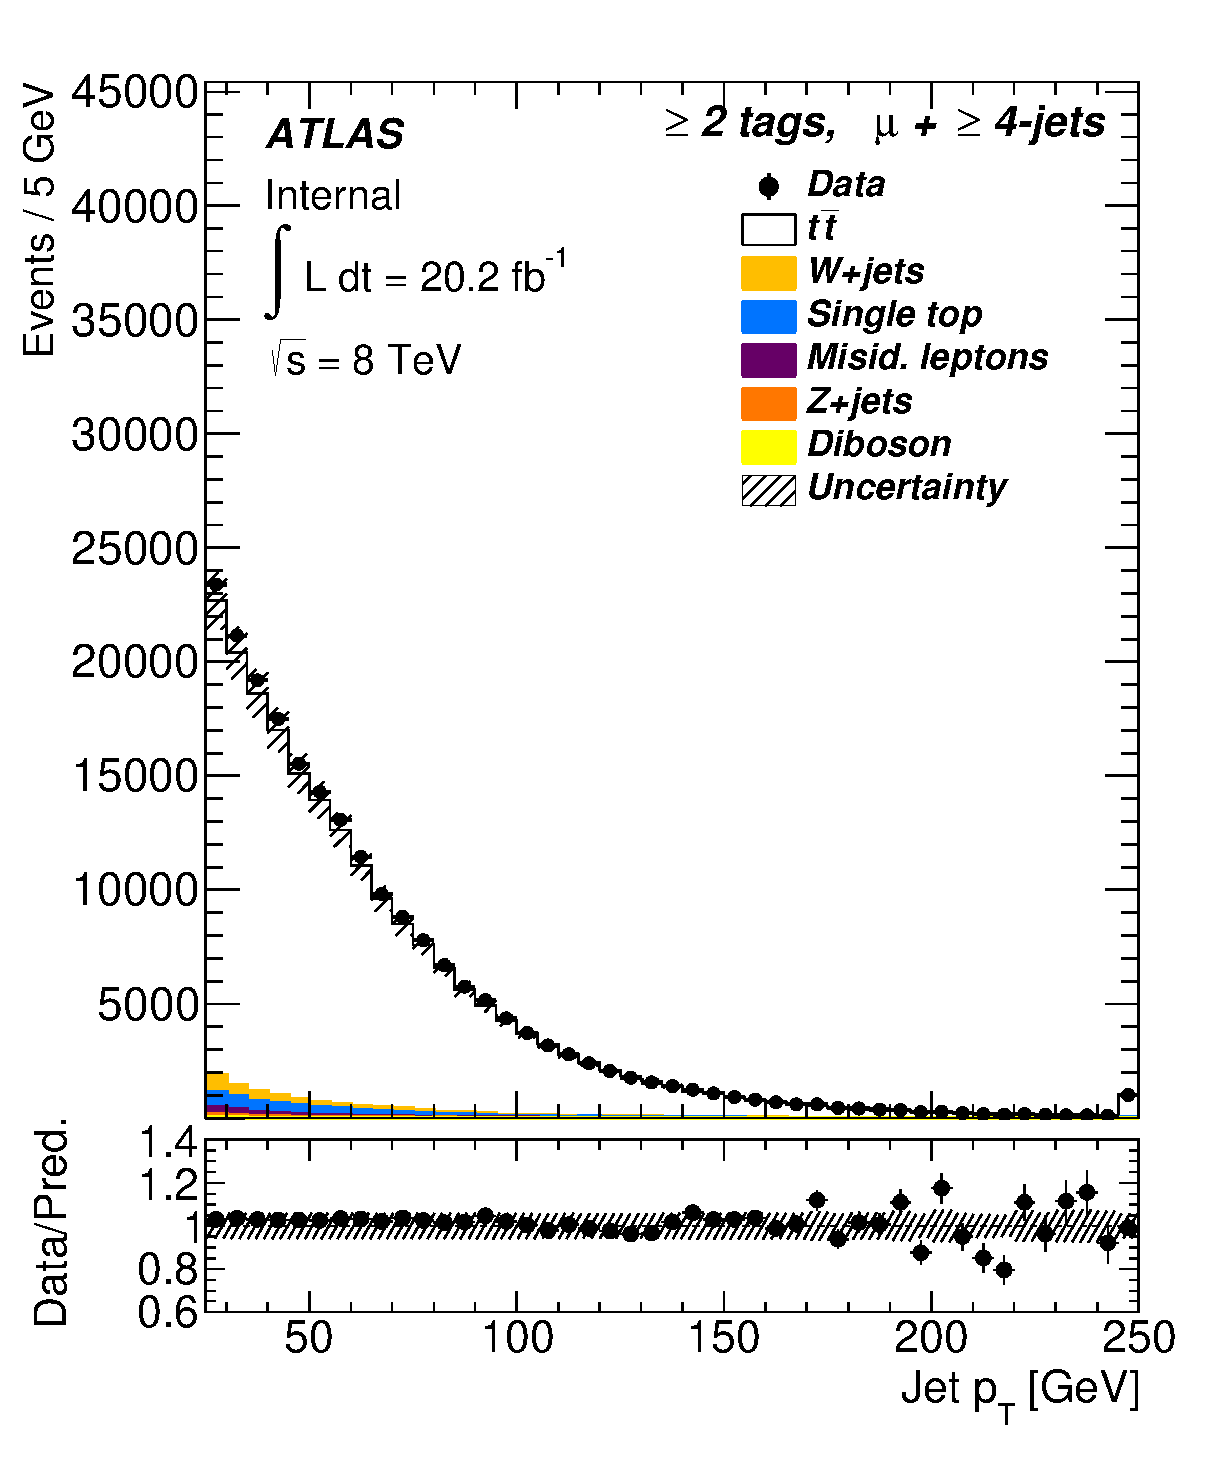
\includegraphics[height=65mm]{chapters/whel/figures/control_Plots2/bTag_2incl/JetPt_mu}\\
		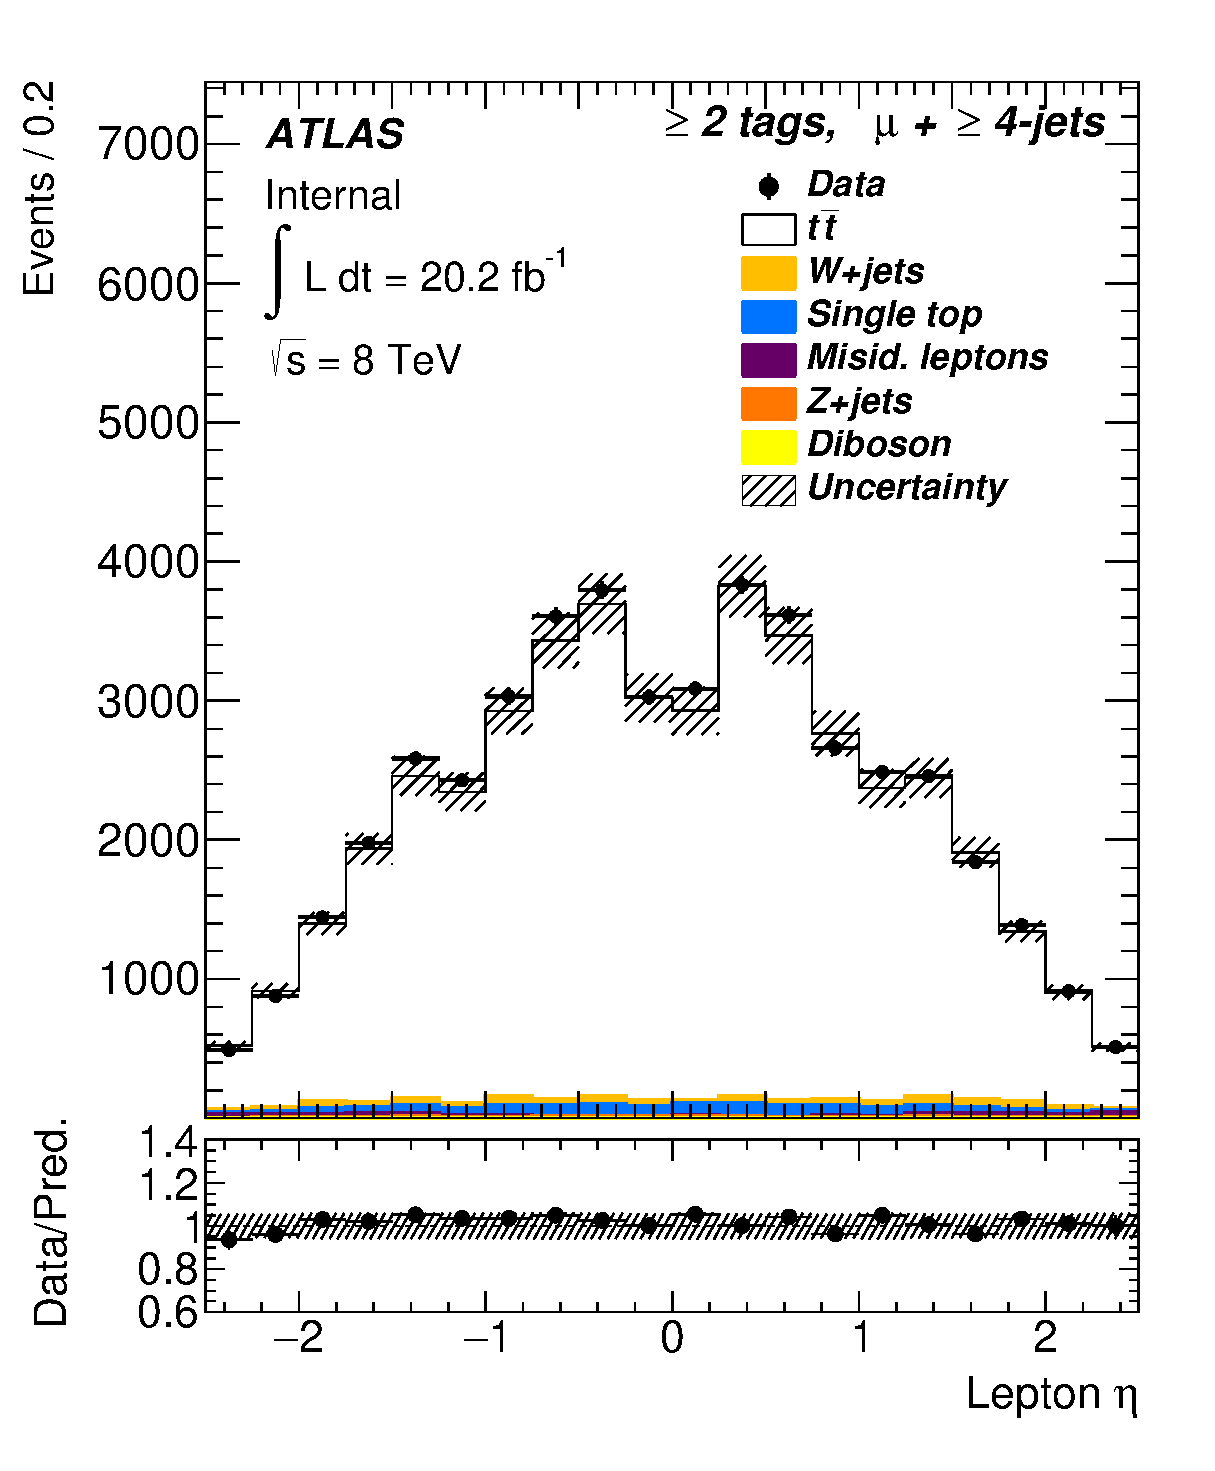
\includegraphics[height=65mm]{chapters/whel/figures/control_Plots2/bTag_2incl/LeptonEta_mu}
		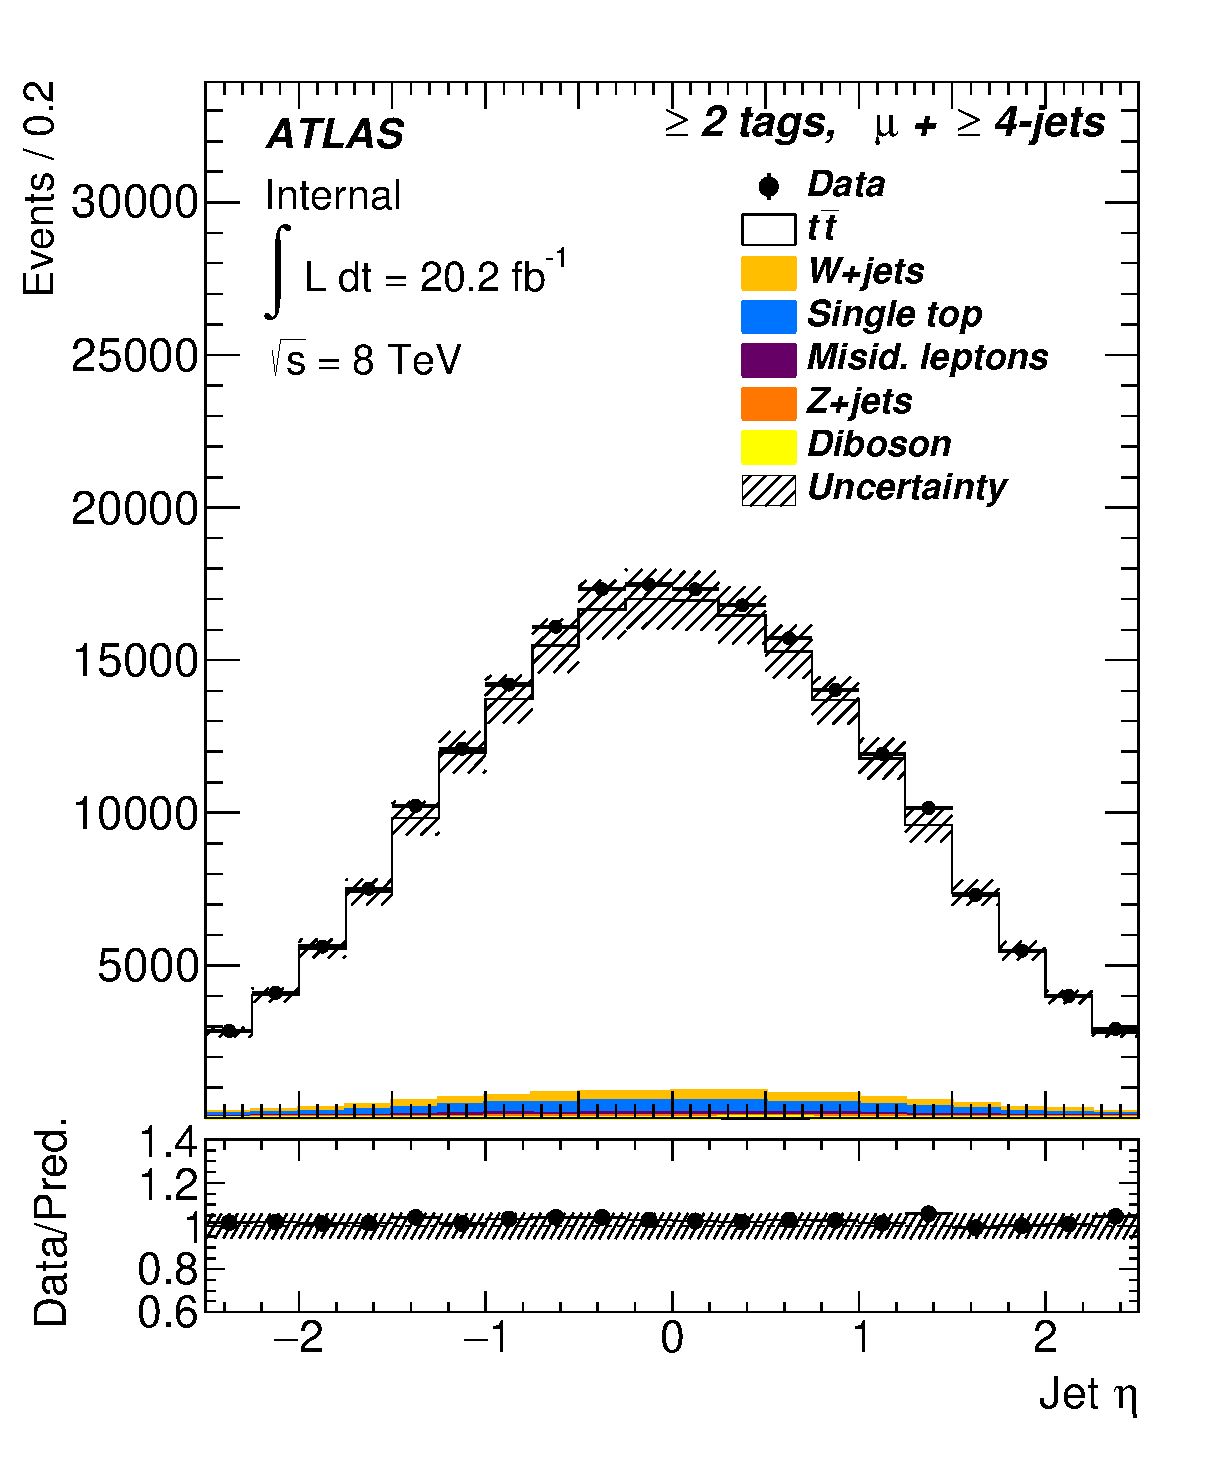
\includegraphics[height=65mm]{chapters/whel/figures/control_Plots2/bTag_2incl/JetEta_mu}\\
		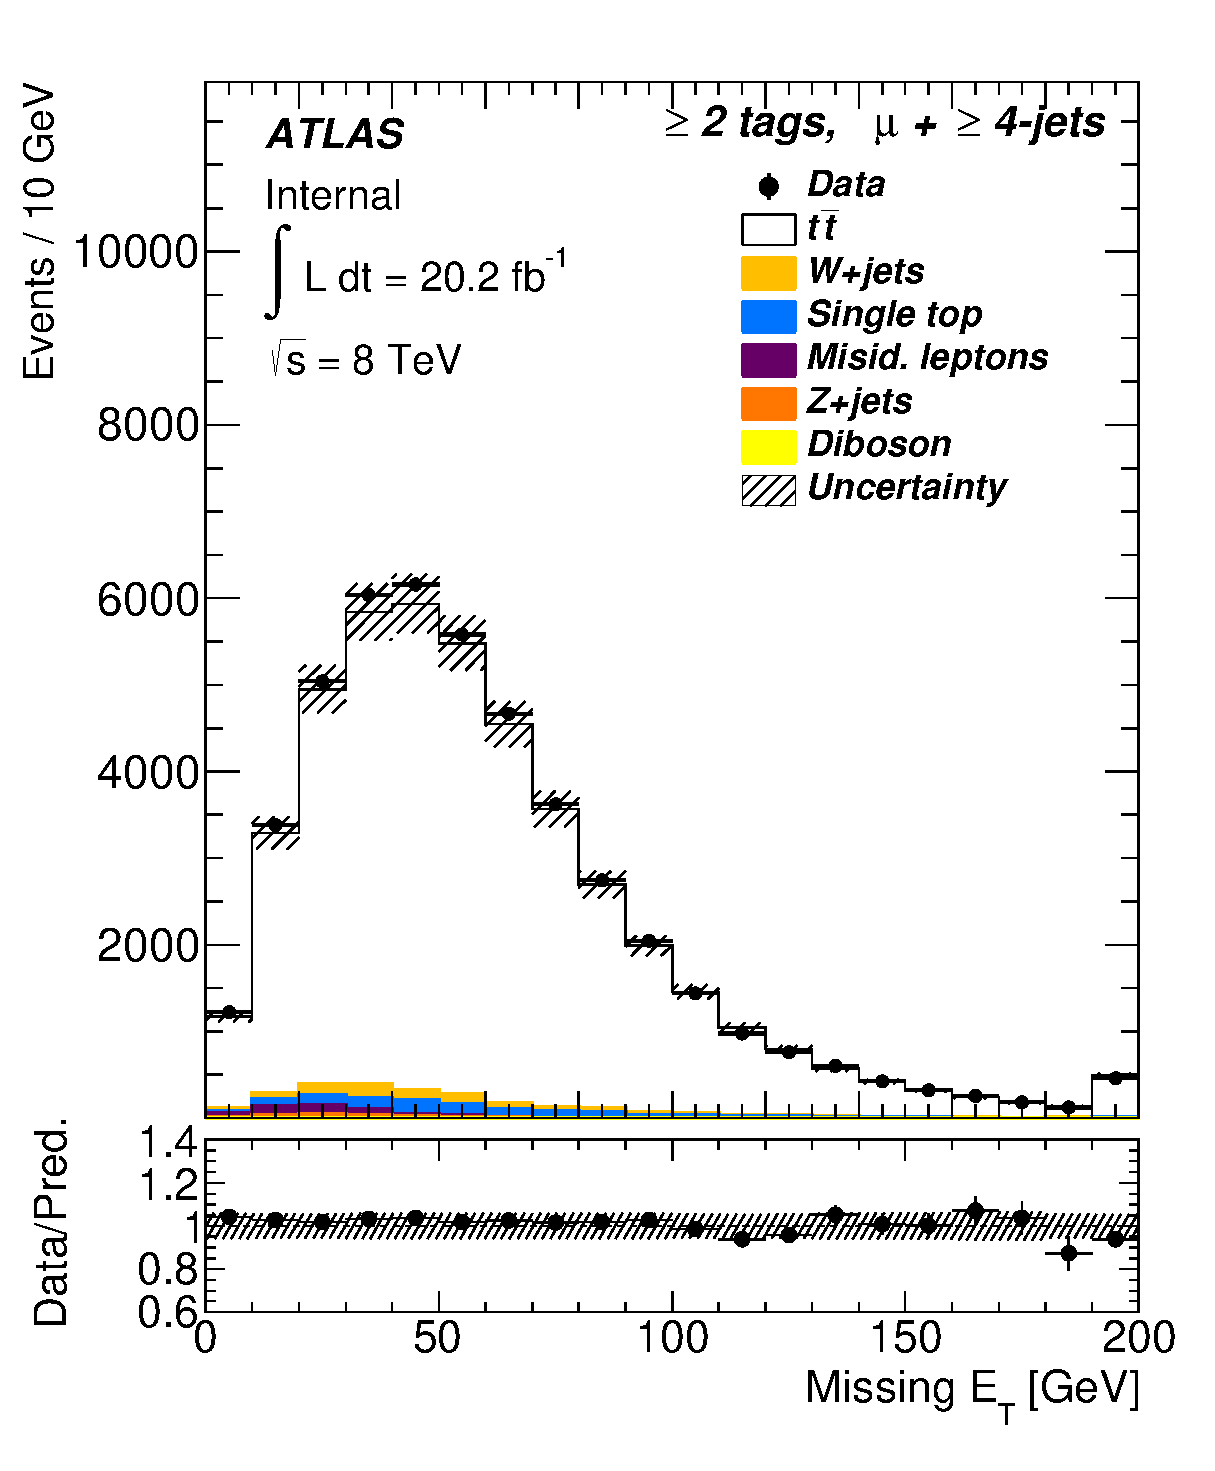
\includegraphics[height=65mm]{chapters/whel/figures/control_Plots2/bTag_2incl/MissingEt_mu}
        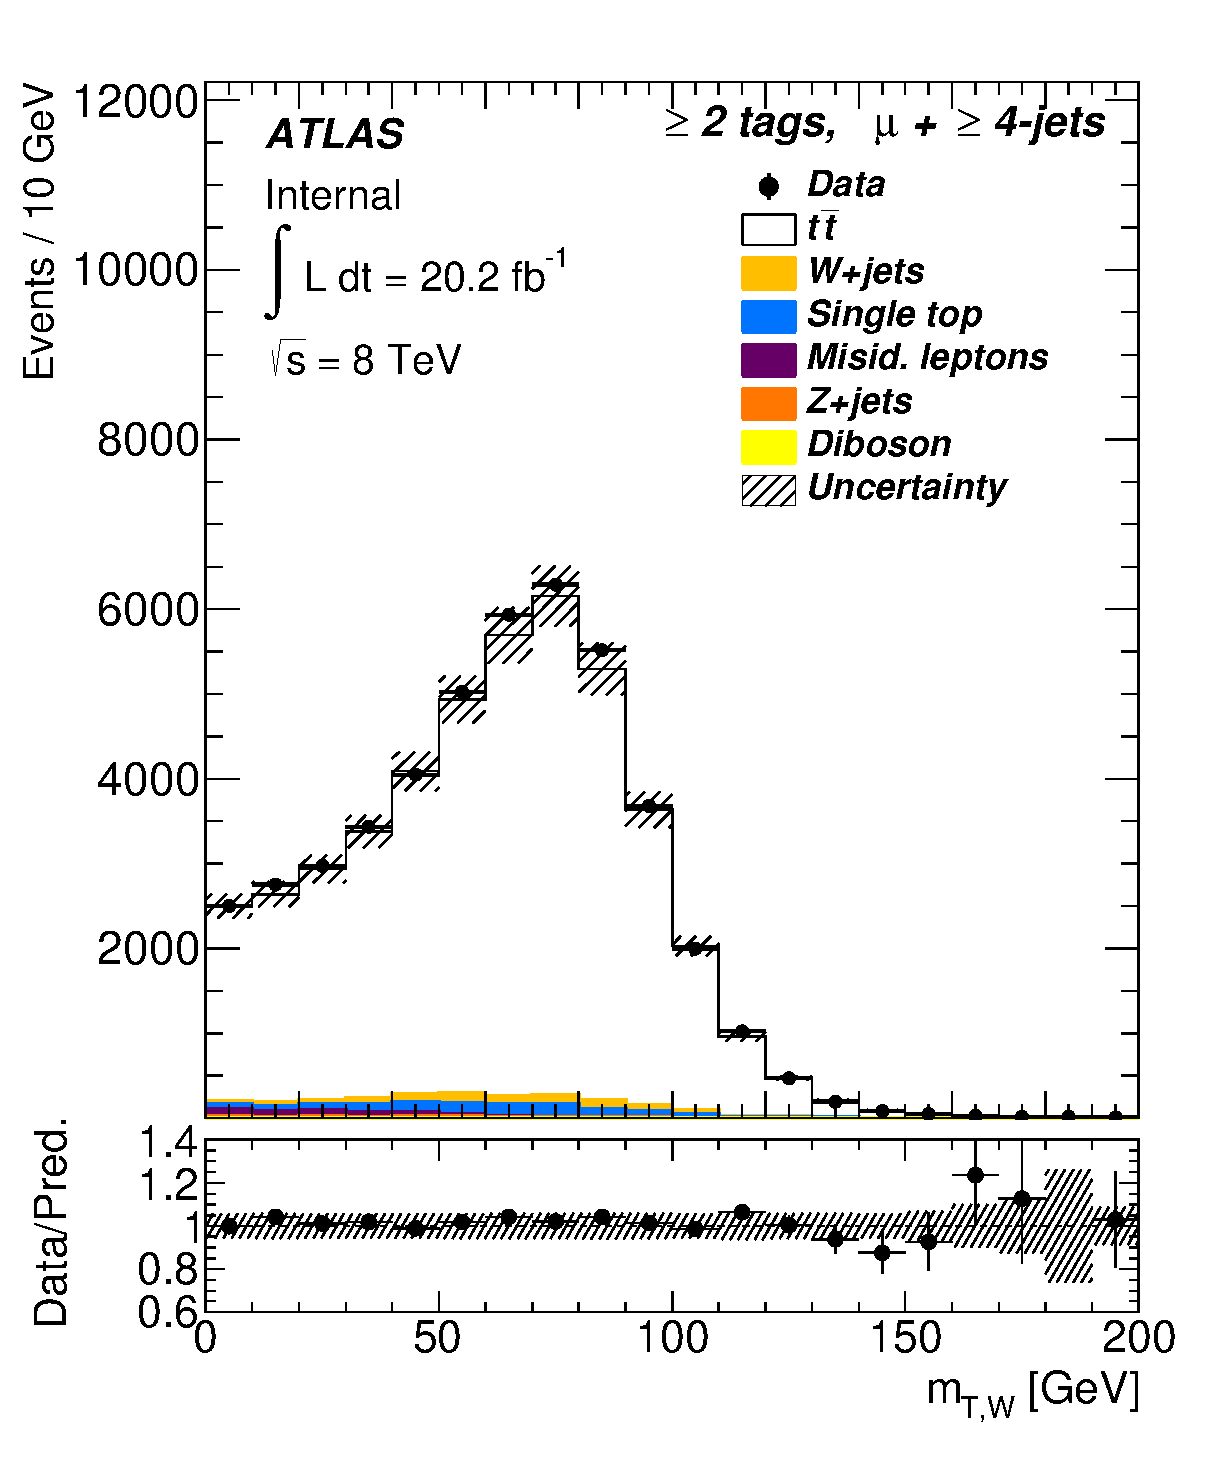
\includegraphics[height=65mm]{chapters/whel/figures/control_Plots2/bTag_2incl/TransverseMass_mu}
	\caption{Plots showing data/MC agreement after event selection for reconstructed objects (lepton, jets, neutrino) in the 2 inclusive \bt tag, muon region. The shaded bands represent the Monte Carlo statistical uncertainties.}
	\label{fig:control_plots_mu_2incl}
	\end{center}
	\end{figure}

\begin{figure}[!hb]
  \begin{center}
    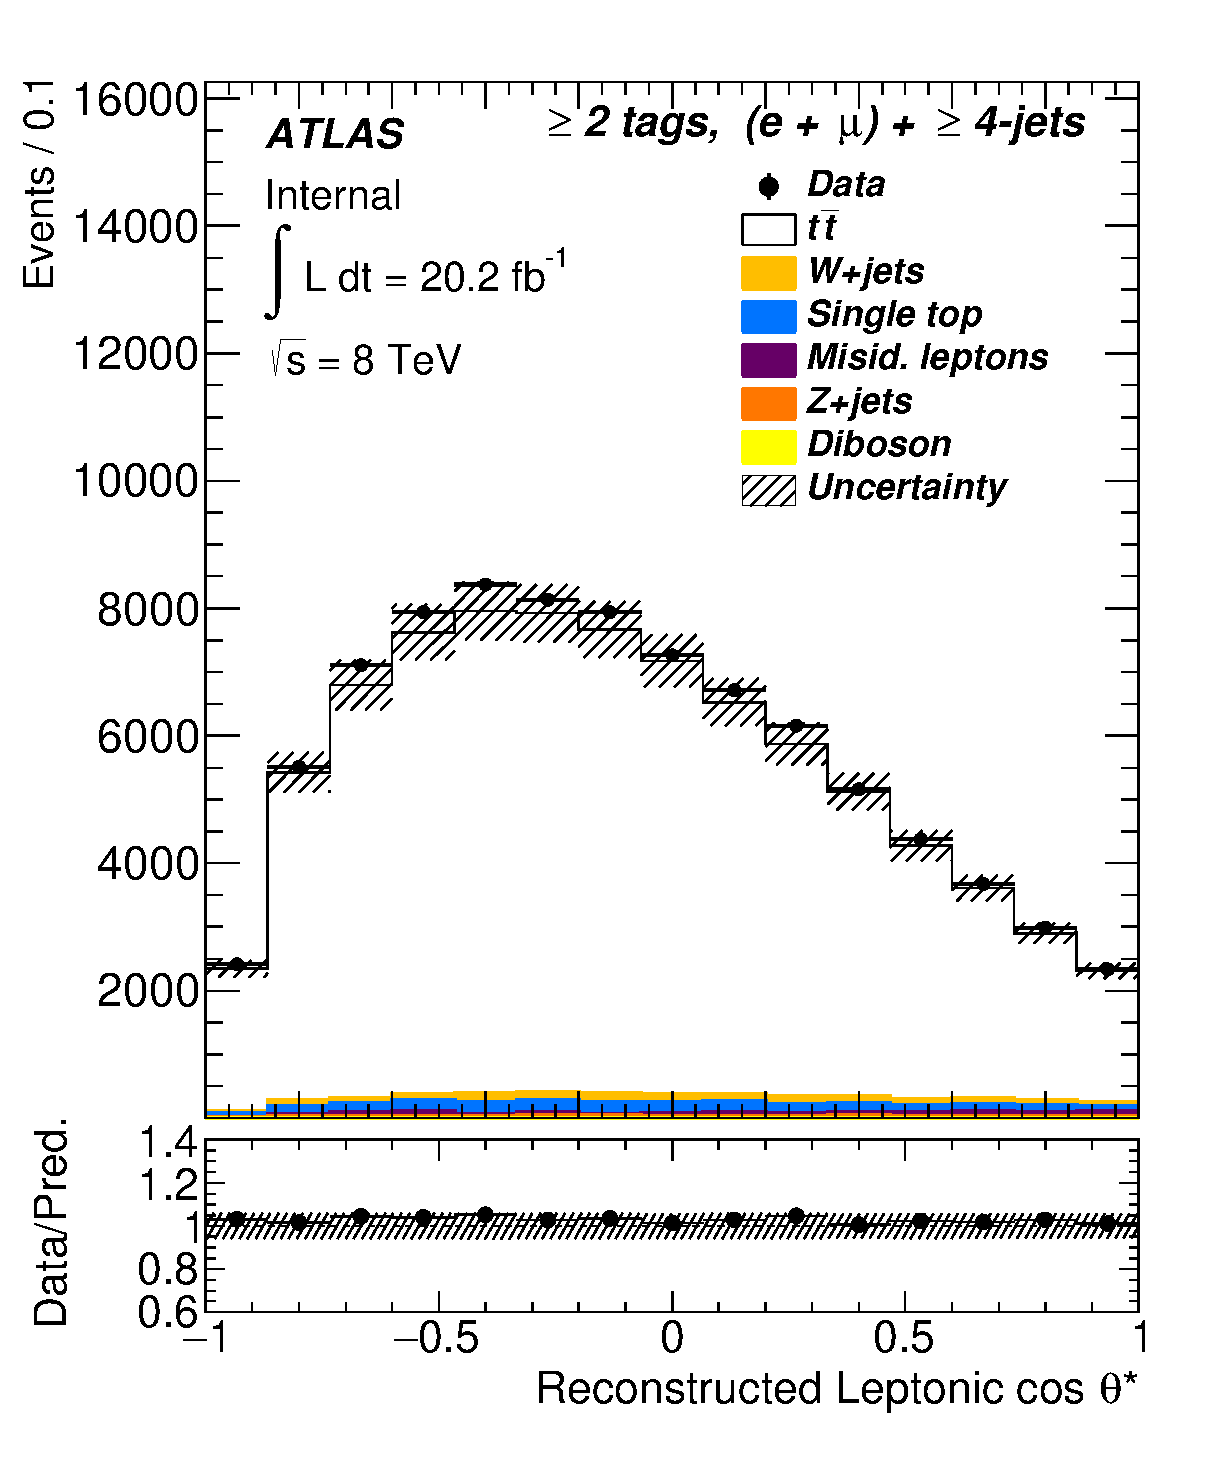
\includegraphics[height=65mm]{chapters/whel/figures/control_Plots2/elmu_2incl_LH48/CosTheta_reco_lep_elmu}
    \includegraphics[height=65mm]{chapters/whel/figures/control_Plots2/elmu_2incl_LH48/CosTheta_reco_had_elmu}\\
    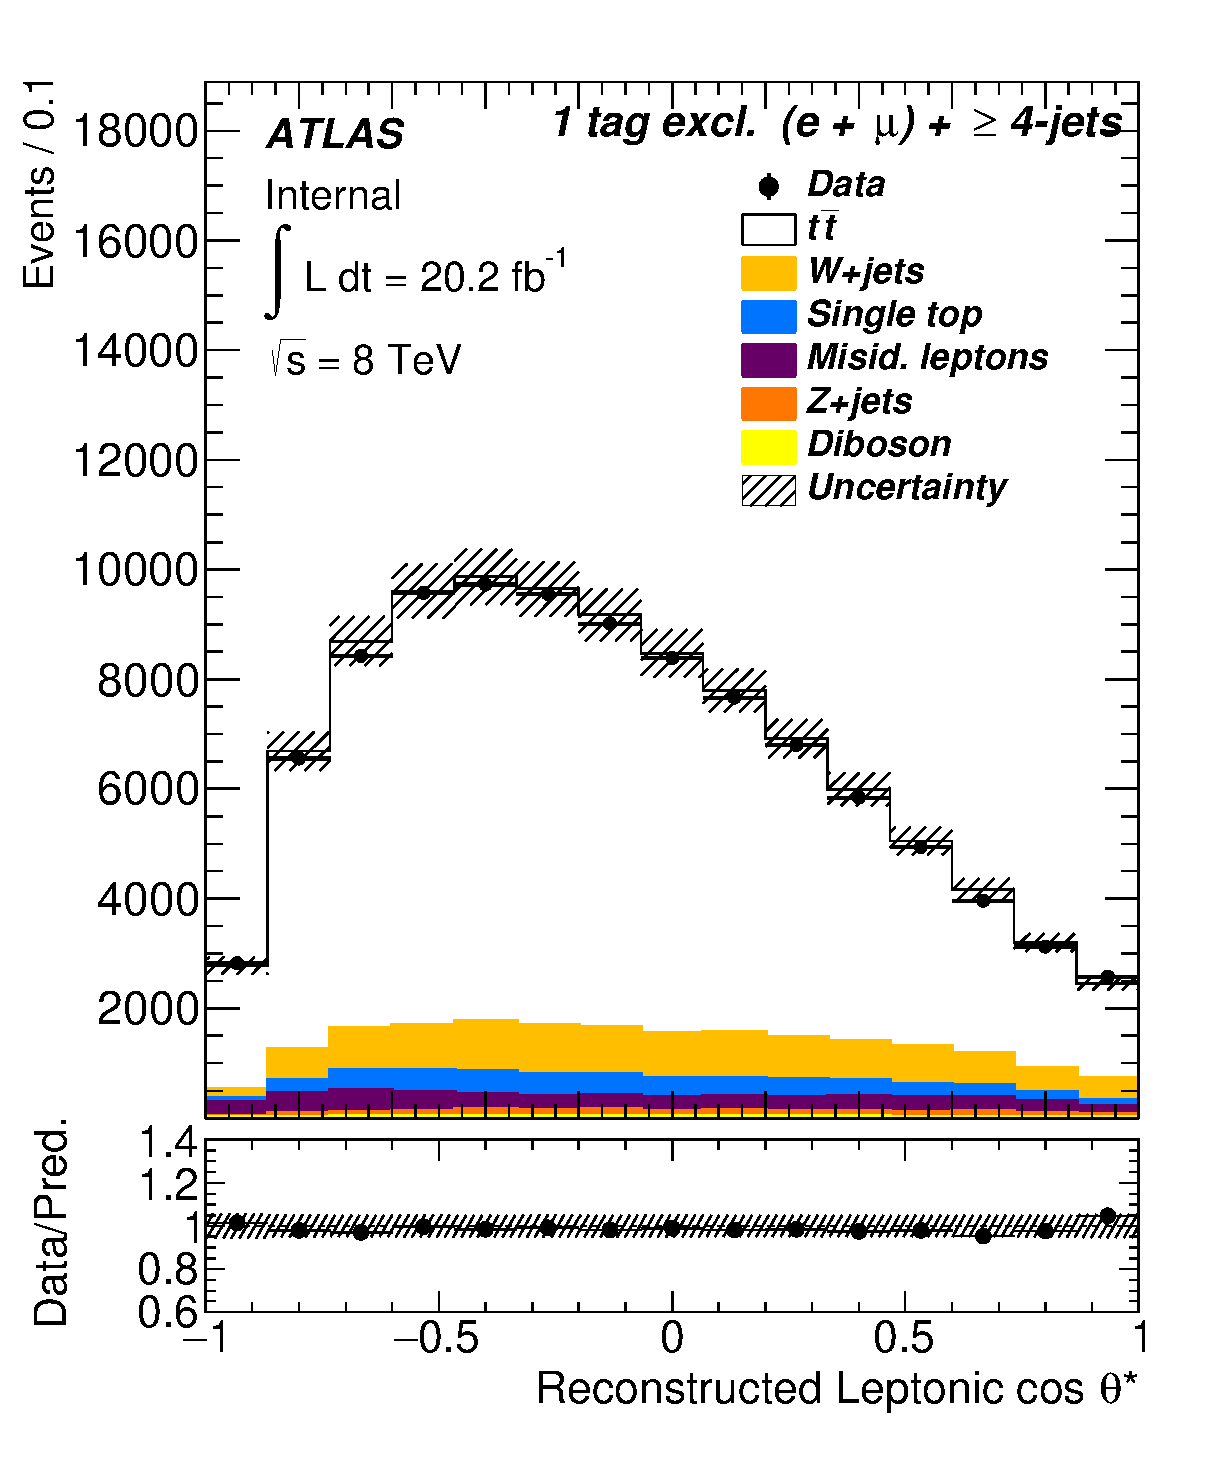
\includegraphics[height=65mm]{chapters/whel/figures/control_Plots2/elmu_1excl_LH48/CosTheta_reco_lep_elmu}
    \includegraphics[height=65mm]{chapters/whel/figures/control_Plots2/elmu_1excl_LH48/CosTheta_reco_had_elmu}
    \caption{Plots showing data/MC agreement after event selection and after the likelihood cut for leptonic and hadronic $\cos\theta^*$ in the 2 inclusive \bt tag (top) and 1 exclusive \bt tag (bottom) region. All plots show merged electron+muon data and Monte Carlo. The shaded bands represent the Monte Carlo statistical uncertainties.}
    \label{fig:control_plots_costheta}
  \end{center}
\end{figure}
\clearpage